% ------------------------------------------------------------------
\renewcommand{\thisunit}{MATH327 Unit 8}
\renewcommand{\moddate}{Last modified 1 Apr.~2022}
\setcounter{section}{8}
\setcounter{subsection}{0}
\phantomsection
\addcontentsline{toc}{section}{Unit 8: Quantum gases}
\section*{Unit 8: Quantum gases}
\subsection{\label{sec:photon}The photon gas}
\subsubsection{Massive bosons in a box}
In \secref{sec:bose} we derived the grand-canonical partition function (\eq{eq:partfunc_BE}) that defines quantum Bose--Einstein statistics for systems of non-interacting bosons,
\begin{equation*}
  \ZBE(\be, \mu) = \prod_{\ell = 0}^{\cL} \frac{1}{1 - e^{-\be (E_{\ell} - \mu)}}.
\end{equation*}
Following the quantum approach, we obtained this result by considering in turn each energy level $\cE_{\ell}$ with energy $E_{\ell}$, and summing over all possible occupation numbers that it could have.
For bosons, $n_{\ell} \in \Nbb_0$ produces sums that only converge if $\mu < E_{\ell}$ for all $\ell$.
The corresponding grand-canonical potential is
\begin{equation*}
  \Phi_{\text{BE}} = -T \log \ZBE = T \sum_{\ell = 0}^{\cL} \log\left[1 - e^{-\be (E_{\ell} - \mu)}\right],
\end{equation*}
from which we can determine the large-scale properties of the system, including its average internal energy $\vev{E}$, average particle number $\vev{N}$, entropy $S$, and pressure $P$.

To do so, we have to specify the energy levels of the particles that compose the system of interest, taking care to note potentially degenerate energy levels $\left\{\cE_m, \cE_n\right\}$ with the same energy $E_m = E_n$ for $m \neq n$.
One example of this that we have already considered is the analysis of non-relativistic ideal gas particles in \secref{sec:regulate}.
For a single particle with mass $m$ in a volume $V = L^3$, we adopted an ansatz for the quantized energies,
\begin{align}
  \label{eq:nonrel_energy}
  E(k_x, k_y, k_z) & = \frac{\hbar^2 \pi^2}{2mL^2}\left(k_x^2 + k_y^2 + k_z^2\right) = \eps \left(k_x^2 + k_y^2 + k_z^2\right) \qquad &
  \eps & \equiv \frac{\hbar^2 \pi^2}{2mL^2},
\end{align}
where the integers $k_{x, y, z}$ specify the possible momenta of the particle,
\begin{align*}
  \vec p & = (p_x, p_y, p_z) = \hbar \frac{\pi}{L} (k_x, k_y, k_z) &
  k_{x, y, z} & = 1, 2, \cdots.
\end{align*}

Compared to \eq{eq:quant_mom}, here we have adjusted our ansatz to require strictly positive $k_{x, y, z}$.
This adjustment is required by another feature of quantum mechanics, which this paragraph will imprecisely describe for the curious.
This description can be skipped without any problem, with the adjusted ansatz simply taken as input.
The feature at play here is known as \href{https://en.wikipedia.org/wiki/Uncertainty_principle}{Heisenberg's uncertainty principle} (named after \href{https://en.wikipedia.org/wiki/Werner_Heisenberg}{Werner Heisenberg}), which relates the precision with which the position and momentum of each particle can simultaneously be \emph{defined}:
\begin{equation*}
  \left(\De x\right) \left(\De p_x\right) \gtrsim \hbar
\end{equation*}
and similarly for $y$ and $z$.
The `$\gtrsim$' sign here hints that we're ignoring irrelevant factors of $2$ and $\pi$, while `$\De$' refers to the precision (or uncertainty) with which $x$ and $p_x$ are defined.
Since the particle is within a volume $V = L^3$, we know $\De x \lesssim L$.
Therefore the uncertainty principle requires $\De p_x \gtrsim \hbar / L$, which is only possible if $p_x$ is non-zero, corresponding to $k_x \geq 1$.
Note that smaller lengths $L$ imply larger momenta and therefore larger energies.

With this adjusted ansatz, $k_{x, y, z} \geq 1$, we can adapt an exercise from \secref{sec:regulate} and ask: What are the lowest energies and the degeneracies of the corresponding energy levels?
\begin{mdframed}
  \ \\[100 pt]
\end{mdframed}

\subsubsection{Massless photons}
Now we will build on our experience with massive bosons to consider a gas of \textit{photons}, massless bosonic quantum particles of light.
For our purposes, with no prior knowledge of particle physics, we can define photons simply by specifying their energy levels.
Clearly $E \propto 1 / m$ from \eq{eq:nonrel_energy} is problematic for massless particles with $m = 0$.
Instead, a photon's energy is proportional to the magnitude of its momentum,
\begin{equation*}
  \Eph(p) = c \sqrt{p_x^2 + p_y^2 + p_z^2} \equiv c p.
\end{equation*}
Here the speed of light $c$ is really just a unit conversion factor (like the Boltzmann constant) that we could set to $c = 1$ by working in appropriate units.

This relation is connected to the non-relativistic energy $E = \frac{p^2}{2m}$ that we considered in \secref{sec:regulate} through the general expression
\begin{equation*}
  E^2 = \left(mc^2\right)^2 + \left(pc\right)^2,
\end{equation*}
which is sometimes called Einstein's triangle.
When $m = 0$, or $m \ll p / c$ more generally, this reproduces the \emph{ultra-relativistic} relation above.
For stationary particles with $p = 0$ it reduces to the famous `mass-energy' $E = mc^2$, while the non-relativistic kinetic energy is recovered for $m \gg p / c$: % TODO: Could add v<<c in this regime, though may lead to confusion if students assume v>>c in the ultra-relativistic regime...
\begin{mdframed}
  \ \\[60 pt] % WARNING: ADJUSTED SIZE BY HAND TO FILL REMAINDER OF PAGE
\end{mdframed}

Another feature of photons' energy levels is that each momentum $(p_x, p_y, p_z)$ corresponds to two degenerate energy levels with the same energy $E(p)$.
This arises from photons' connection to electric and magnetic fields, which allows each photon to be \href{https://en.wikipedia.org/wiki/Photon_polarization}{polarized} in two different ways.
If there is interest we can discuss this further in a tutorial, but it is not relevant to the statistical physics of photons, for which we can take this double degeneracy as input.
Note that this factor of two multiplies all other degeneracies, for instance from permutations of $(p_x, p_y, p_z)$.

For photons in a volume $V = L^3$, only the same discrete momenta as in the massive case are allowed,
\begin{align*}
  p & = \hbar \frac{\pi}{L} \sqrt{k_x^2 + k_y^2 + k_z^2} \equiv \hbar \frac{\pi}{L} k &
  k_{x, y, z} = 1, 2, \cdots,
\end{align*}
so that the quantized photon energies are
\begin{equation}
  \label{eq:photon_Ek}
  \Eph(k) = \hbar c \frac{\pi}{L} k.
\end{equation}
Because light is an electromagnetic wave, it is convenient to work in terms of photons' wavelength \la and angular frequency $\om = 2\pi f$ (not to be confused with generic micro-states $\om_i$).
Together, the wavelength and frequency determine the speed of the wave's propagation, in this case the speed of light % TODO: In vacuum, or at least linear medium...
\begin{equation*}
  c = \frac{\la \om}{2\pi}.
\end{equation*}

In quantum physics, a particle's momentum is related to its de~Broglie wavelength, implying that in a volume $V = L^3$ the wavelengths are also quantized as illustrated in the picture below (from Schroeder's \textit{Introduction to Thermal Physics}).
Specifically, the length $L$ must be an integer multiple of half a wavelength,
\begin{equation*}
  L = k \frac{\la}{2} \qquad \Lra \qquad c = \frac{L}{k} \frac{\om}{\pi} = \frac{\om}{\frac{\pi}{L} k},
\end{equation*}
and we can rewrite \eq{eq:photon_Ek} as
\begin{equation}
  \label{eq:photon_omega}
  \Eph(\om) = \hbar \om.
\end{equation}
With $\la \propto c / \om$, this incorporates the relation between length and energy scales that we noted above.
Low (\textit{infrared}) frequencies correspond to small energies and long wavelengths, while high (\textit{ultraviolet}) frequencies correspond to large energies and short wavelengths. \\[-24 pt]
\begin{center}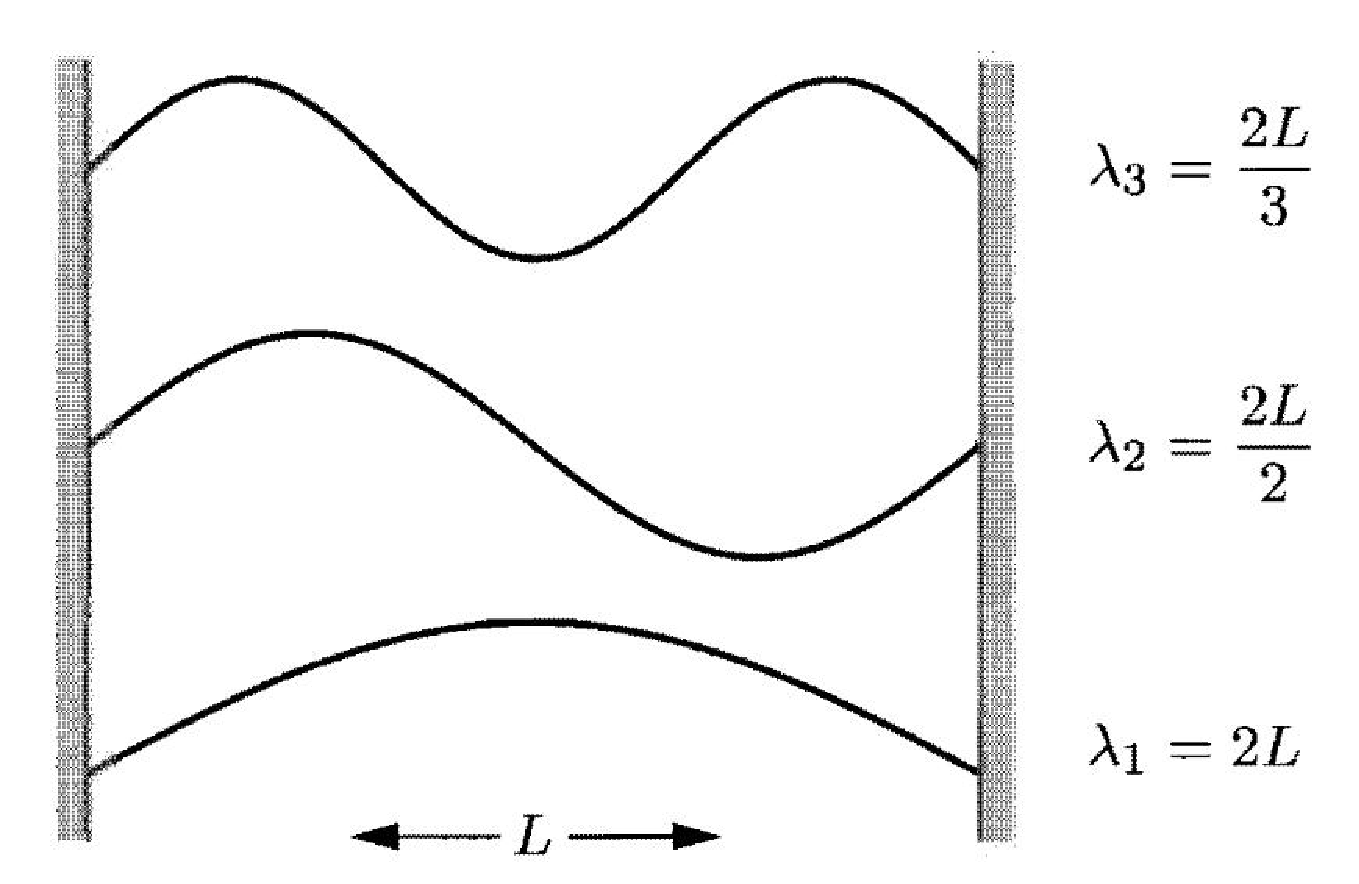
\includegraphics[width=0.65\textwidth]{figs/unit08_wavelengths.pdf}\end{center} % WARNING: ADJUSTED SIZE BY HAND TO FILL REMAINDER OF PAGE

We are now ready to write down the grand-canonical potential for a photon gas:
\begin{equation*}
  \Phi_{\text{ph}} = T \sum_{\ell = 0}^{\cL} \log\left[1 - e^{-\be (E_{\ell} - \mu)}\right] = 2T \sum_{\vec k} \log\left[1 - e^{-\be (\Eph(k) - \mu)}\right],
\end{equation*}
where the factor of $2$ in the final expression accounts for the doubly degenerate energy levels.
We can simplify this expression by appreciating that photons are easy to create and destroy.
Every time a light is switched on, it begins emitting a constant flood of photons (with wavelengths of several hundred nanometres).
Food in a microwave oven gets hot by absorbing many lower-energy photons (with longer wavelengths around $12$~centimetres).
In both cases an enormous number of photons is required to make even a small change in energy, so that \eq{eq:mu_E} implies the chemical potential of a photon gas must be negligible,
\begin{equation*}
  \mu = \left.\pderiv{E}{N}\right|_S \approx 0 \qquad \Lra \qquad \Phi_{\text{ph}} \approx 2T \sum_{\vec k} \log\left[1 - e^{-\be \Eph(k)}\right].
\end{equation*}
% TODO: Can emphasize that particle number still fluctuating greatly, despite (in fact, because of) chemical potential no longer appearing in expression...
Since we have $k_{x, y, z} \geq 1$, the strictly positive energies $\Eph(k) \propto k / L > 0$ ensure Bose--Einstein statistics is still convergent even with $\mu = 0$.

Another simplification comes from considering the photon gas in a large volume, so that the energies $\Eph(k) \propto k / L$ are very closely spaced and we can approximate the sum over integer $k_{x, y, z}$ by integrals over continuous real $\khat_{x, y, z}$, % TODO: Mention Poisson resummation?...
\begin{equation*}
  \Phi_{\text{ph}} \approx 2T \int d\khat_x \; d\khat_y \; d\khat_z \; \log\left[1 - e^{-\be \Eph(\khat)}\right].
\end{equation*}
Since the energy $\Eph(\khat)$ depends only on the magnitude $\khat$, we can profit from converting to spherical coordinates.
When we do so, we have to keep in mind that $k_{x, y, z} > 0$ corresponds only to the positive octant of the sphere, % TODO: Explicitly justify setting lower bounds to zero?...
\begin{equation*}
  \int_0^{\infty} d\khat_x \int_0^{\infty} d\khat_y \int_0^{\infty} d\khat_z = \int_0^{\infty} d\khat \; \khat^2 \int_0^{\pi / 2} d\theta \; \sin\theta \int_0^{\pi / 2} d\phi = \frac{\pi}{2} \int_0^{\infty} d\khat \; \khat^2,
\end{equation*}
so that
\begin{equation*}
  \Phi_{\text{ph}} \approx \pi T \int_0^{\infty} d\khat \; \khat^2 \log\left[1 - e^{-\be \Eph(\khat)}\right].
\end{equation*}
We can finally change variables to integrate over the photon angular frequency $\om = c \frac{\pi}{L} k$, with $\Eph = \hbar \om$, to find
\begin{align}
  \Phi_{\text{ph}} & \approx \pi T \left(\frac{L}{c \pi}\right)^3 \int_0^{\infty} d\om \; \om^2 \log\left[1 - e^{-\be \hbar \om}\right] \cr
                   & = \frac{VT}{c^3 \pi^2} \int_0^{\infty} d\om \; \om^2 \log\left[1 - e^{-\be \hbar \om}\right], \label{eq:photon_grand}
\end{align}
recognizing $L^3 = V$.
With this grand-canonical potential derived, we just need to take the appropriate derivatives to determine the thermodynamics and equation of state for the photon gas.
% ------------------------------------------------------------------



% ------------------------------------------------------------------
\subsection{\label{sec:planck}The sun and the void}
It will be very interesting to use the grand-canonical potential in \eq{eq:photon_grand} to analyze the average internal energy for a photon gas.
With $\mu = 0$, \eq{eq:E_grand} from \secref{sec:grand_pot} becomes
\begin{equation*}
  \vev{E}_{\text{ph}} = -T^2 \pderiv{}{T} \left[\frac{\Phi_{\text{ph}}}{T}\right] = \pderiv{}{\be} \left[\be \Phi_{\text{ph}}\right].
\end{equation*}
To begin, we will consider the energy density expressed as an integral over photon frequencies,
\begin{equation*}
  \frac{\vev{E}_{\text{ph}}}{V} = \int_0^{\infty} P(\om) \; d\om,
\end{equation*}
where the function $P(\om)$ is known as the \textit{spectral density}, or simply the \textit{spectrum}.
(It's not the pressure!)
What is the spectrum for a photon gas?
\begin{mdframed}
  $\displaystyle \frac{\vev{E}_{\text{ph}}}{V} = \frac{1}{c^3 \pi^2} \int_0^{\infty} d\om \; \om^2 \pderiv{}{\be} \log\left[1 - e^{-\be \hbar \om}\right] = $ \\[120 pt] % WARNING: FORMATTING BY HAND
\end{mdframed}

You should find
\begin{equation}
  \label{eq:Planck_omega}
  P(\om) = \left(\frac{\hbar}{c^3 \pi^2}\right) \frac{\om^3}{e^{\be \hbar \om} - 1},
\end{equation}
which is known as the Planck spectrum, named after Max Planck.
We can equally well consider the Planck spectrum $P(\la)$ as a function of the wavelength $\la = 2\pi c / \om$, by changing variables in the expression above:
\begin{mdframed}
  $\displaystyle \frac{\vev{E}_{\text{ph}}}{V} = \frac{\hbar}{c^3 \pi^2} \int_0^{\infty} \frac{\om^3}{e^{\be \hbar \om} - 1} \; d\om = $ \\[120 pt] % WARNING: FORMATTING BY HAND
\end{mdframed}

You should find
\begin{equation}
  \label{eq:Planck_la}
  P(\la) = \left(\frac{16\pi^2 \hbar c}{\la^5}\right) \frac{1}{e^{2\pi\be \hbar c / \la} - 1},
\end{equation}
which is plotted for three temperatures $T = 1 / \be$ in the figure below, which comes from \href{https://commons.wikimedia.org/wiki/File:Black_body.svg}{Wikimedia Commons}.
(The plot divides our $P(\la)$ by $4\pi$~steradian and multiplies it by $c$ to convert from a spectral density to a spectral power per unit area per unit of solid angle.  For our purposes only the functional form is significant.)

\begin{center}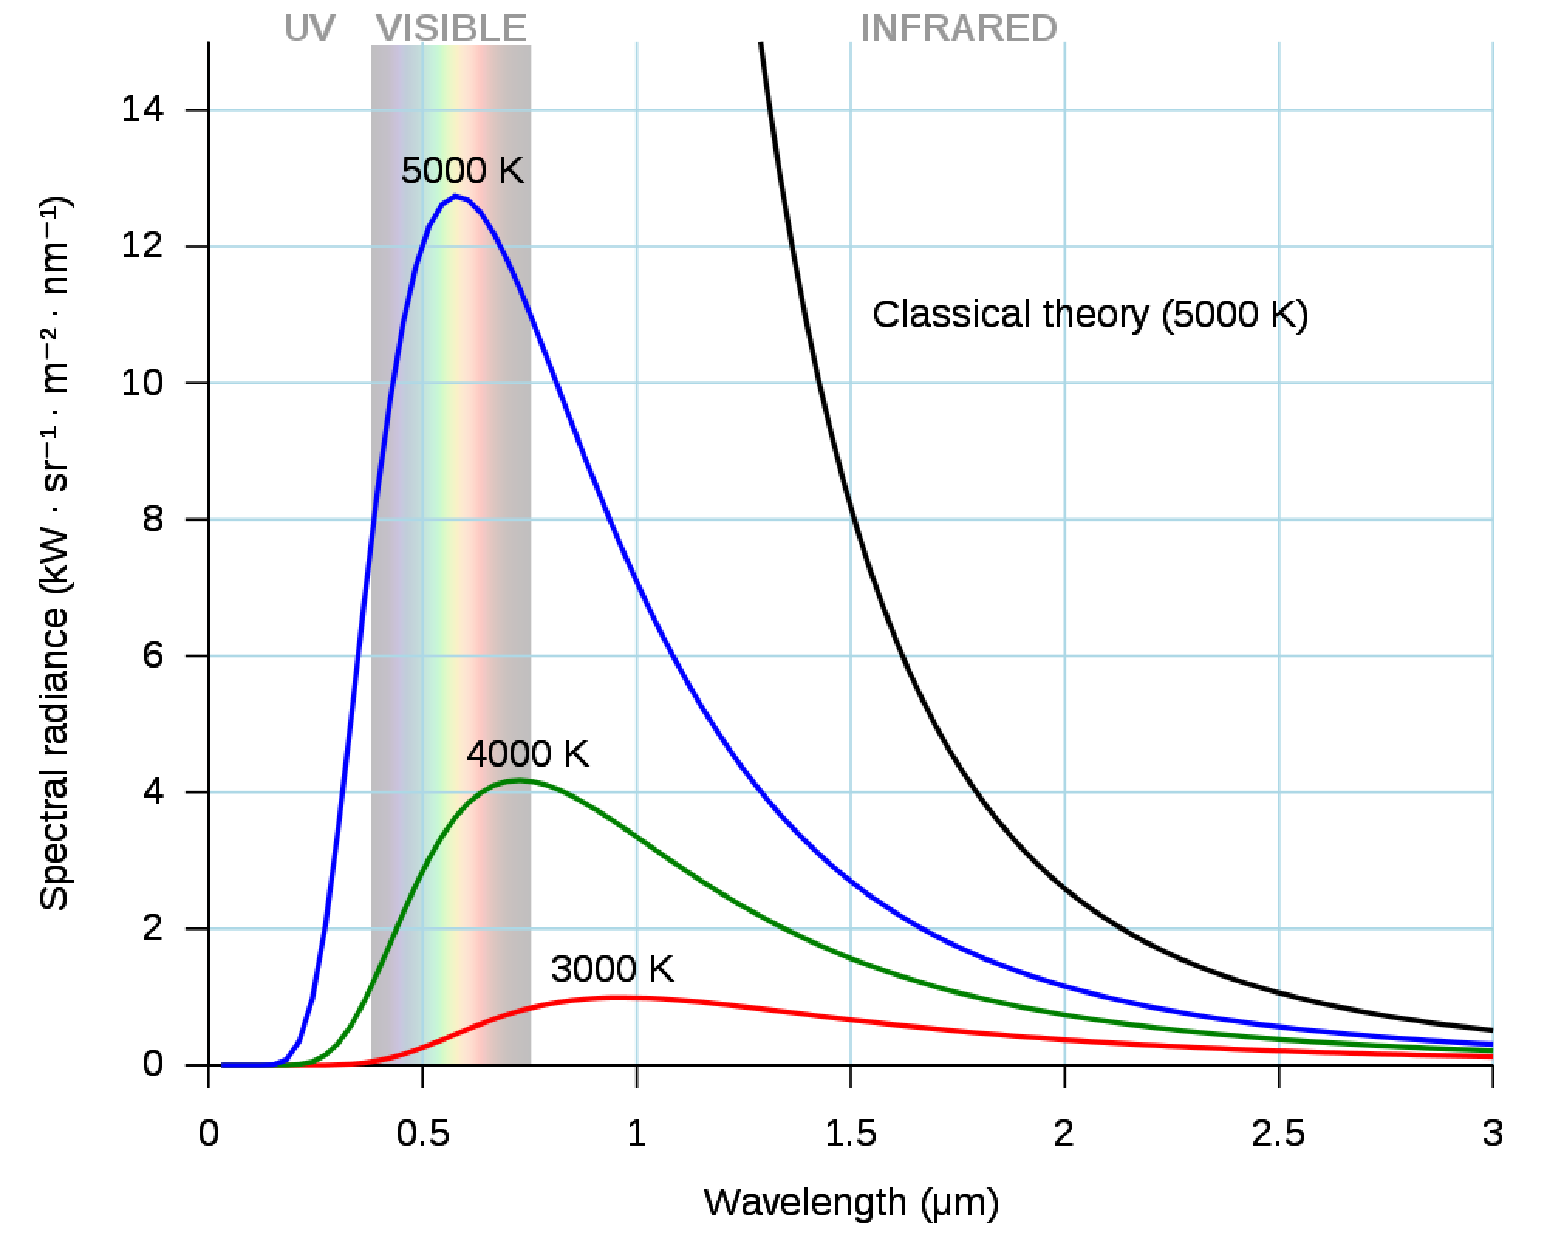
\includegraphics[width=\textwidth]{figs/unit08_spectrum.pdf}\end{center}

Considering first the high-energy ultraviolet (UV) limit of small wavelengths $\la$, we can see from \eq{eq:Planck_la} that $P(\la)$ is exponentially suppressed, which overwhelms the diverging factor $\propto 1 / \la^5$ in parentheses.
In the low-energy infrared limit, the large $\la$ has the same effect that a large temperature ($\be \ll 1$) would have: $e^{2\pi\be \hbar c / \la} - 1 \approx 2\pi\be \hbar c / \la$ and
\begin{equation*}
  P(\la) \approx \left(\frac{16\pi^2 \hbar c}{\la^5}\right) \frac{\la}{2\pi\be \hbar c} = \frac{8\pi T}{\la^4}.
\end{equation*}
The connection to large temperatures indicates that this is what classical statistics would predict for the spectrum of light.
It is known as the Rayleigh--Jeans spectrum, named after \href{https://en.wikipedia.org/wiki/John_William_Strutt,_3rd_Baron_Rayleigh}{the third Baron Rayleigh} and \href{https://en.wikipedia.org/wiki/James_Jeans}{James Jeans}.
Recall that the classical approach sums over all possible energies for each degree of freedom, corresponding to a light-emitting object (historically known as a \textit{black body}) emitting light of all wavelengths $\la$.
According to the classical Rayleigh--Jeans spectrum, in the limit $\la \to 0$ this light would carry an infinite amount of energy, an obvious problem that became known as the \textit{ultraviolet catastrophe}.
Planck described his 1900 derivation of the UV-suppressed $P(\la)$ as ``an act of desperation'' to avoid this problem; it turned out to be one of the first steps towards the quantum physics.

Another noteworthy feature of the Planck spectrum shown above is that as the temperature increases, the maximum of $P(\la)$ moves to shorter wavelengths and correspondingly larger energies.
The fact that the peak of the spectrum for $T \approx 5000$~K falls within the wavelengths of visible light (roughly $400$--$700$~nm) is not a coincidence.
As shown in the figure below, also from \href{https://commons.wikimedia.org/wiki/File:Solar_spectrum_en.svg}{Wikimedia Commons}, the amount of sunlight that reaches the surface of the earth is also maximized around visible wavelengths, which are visible to us because we have evolved to make the most efficient use of this sunlight.

Taking into account the absorption of some sunlight by molecules in the atmosphere, we can see from the figure below that the energy spectrum of the sunlight reaching the top of the atmosphere is quite close to a Planck (or `blackbody') spectrum with temperature $T \approx 5778$~K.
The agreement isn't perfect, which is to be expected since the Planck spectrum relies on the non-trivial assumption of an ideal gas of non-interacting particles.
Despite that caveat, numerically fitting the measured sunlight to the Planck spectrum is how this `effective' surface temperature of the sun is determined.
This same fitting procedure can even be done for distant stars, with red stars corresponding to relatively low temperatures $T \lesssim 3500$~K and blue stars corresponding to relatively high temperatures $T \gtrsim 10{,}000$~K.

\begin{center}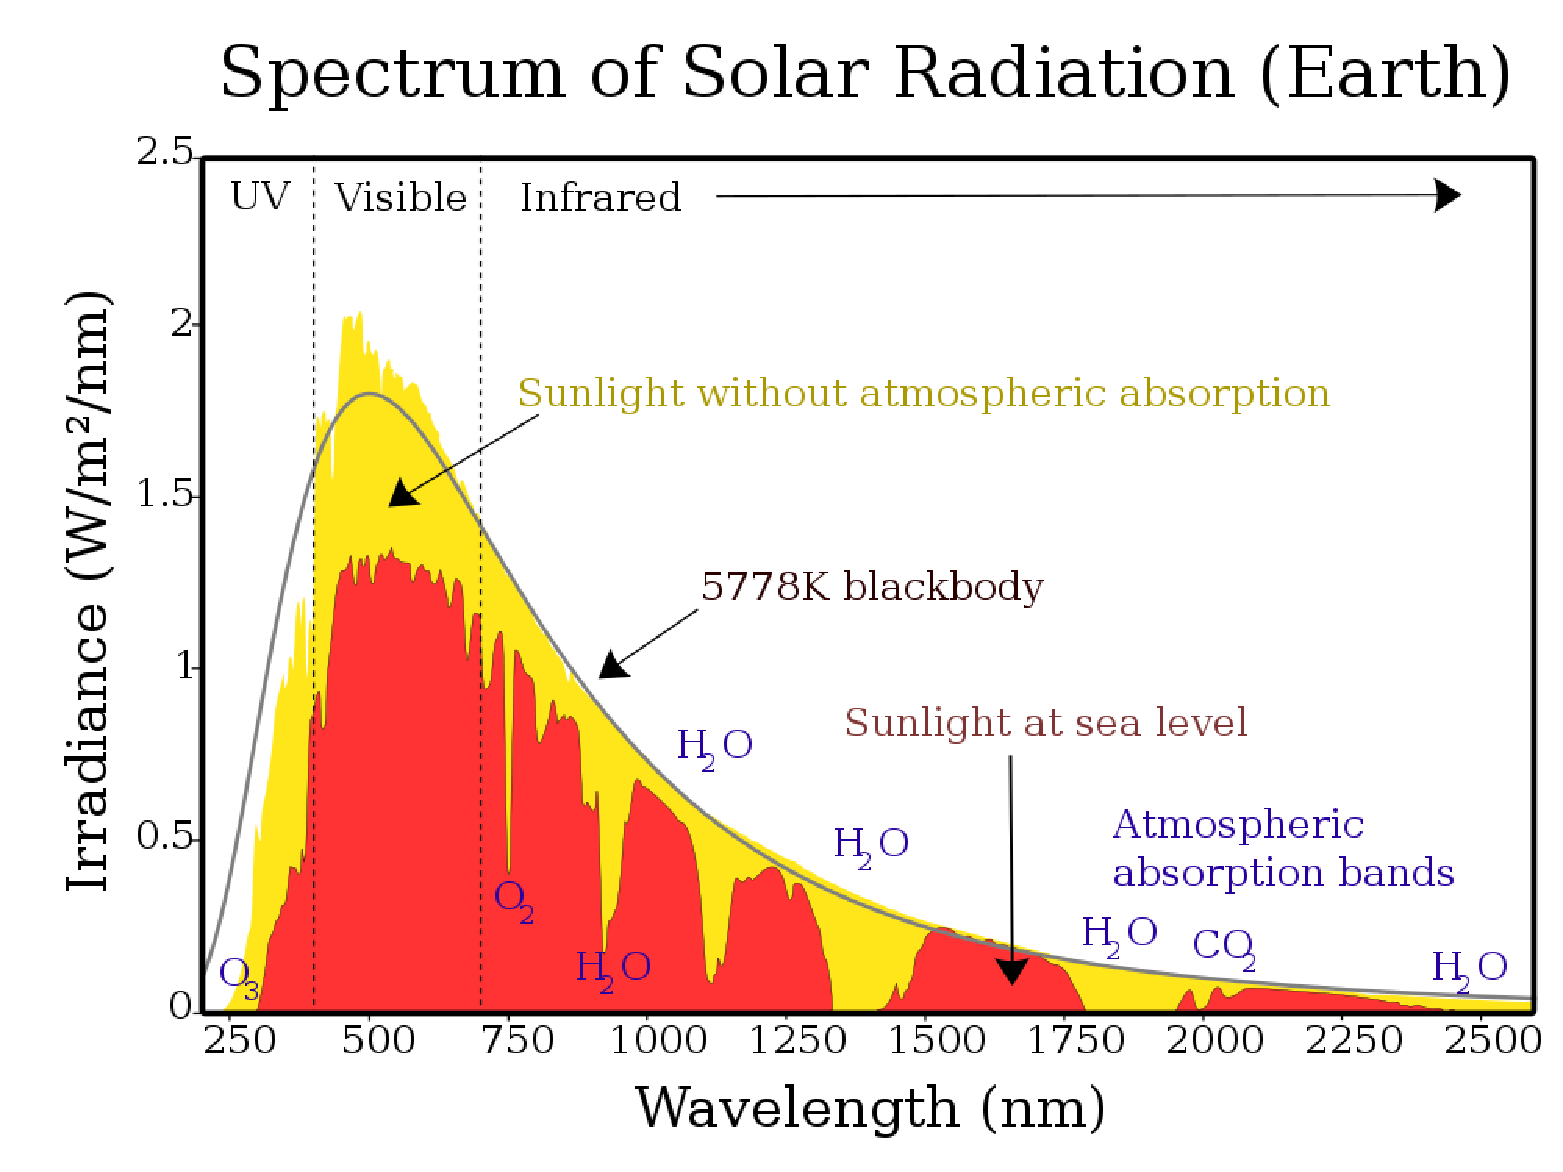
\includegraphics[width=0.9\textwidth]{figs/unit08_sun.pdf}\end{center} % WARNING: ADJUSTED SIZE BY HAND TO FILL REMAINDER OF PAGE

Even more remarkably, we can use the Planck spectrum to determine the temperature of intergalactic space.
Rather than being empty, these voids are actually permeated by a very low-temperature photon gas left over from the Big Bang roughly $14$~billion years ago.
This photon gas is known as the \href{https://en.wikipedia.org/wiki/Cosmic_microwave_background}{cosmic microwave background} (CMB), and carries information about the early evolution of the universe, including some of the strongest evidence for the existence of dark matter.

The picture below is a famous visualization of the CMB, provided by the \href{http://www.esa.int/ESA_Multimedia/Images/2013/03/Planck_CMB}{European Space Agency} and produced from measurements taken by their `Planck' satellite. % Can compare with WMAP from wmap.gsfc.nasa.gov/media/101080/
To produce this image, for each point in the sky the satellite measures the photon spectrum reaching it from that direction.
The contributions coming from stars and galaxies are subtracted, and the remaining data is fit to the Planck spectrum to find the temperature of the intergalactic CMB photon gas at that point.
From point to point, there are only small temperature fluctuations around the average $T_{\text{CMB}} \approx 2.725$~K.
That average temperature is subtracted and the fluctuations themselves are shown below, with warmer red-coloured regions only $\De T \approx 0.0002$~K hotter than the cooler blue-coloured regions.

\begin{center}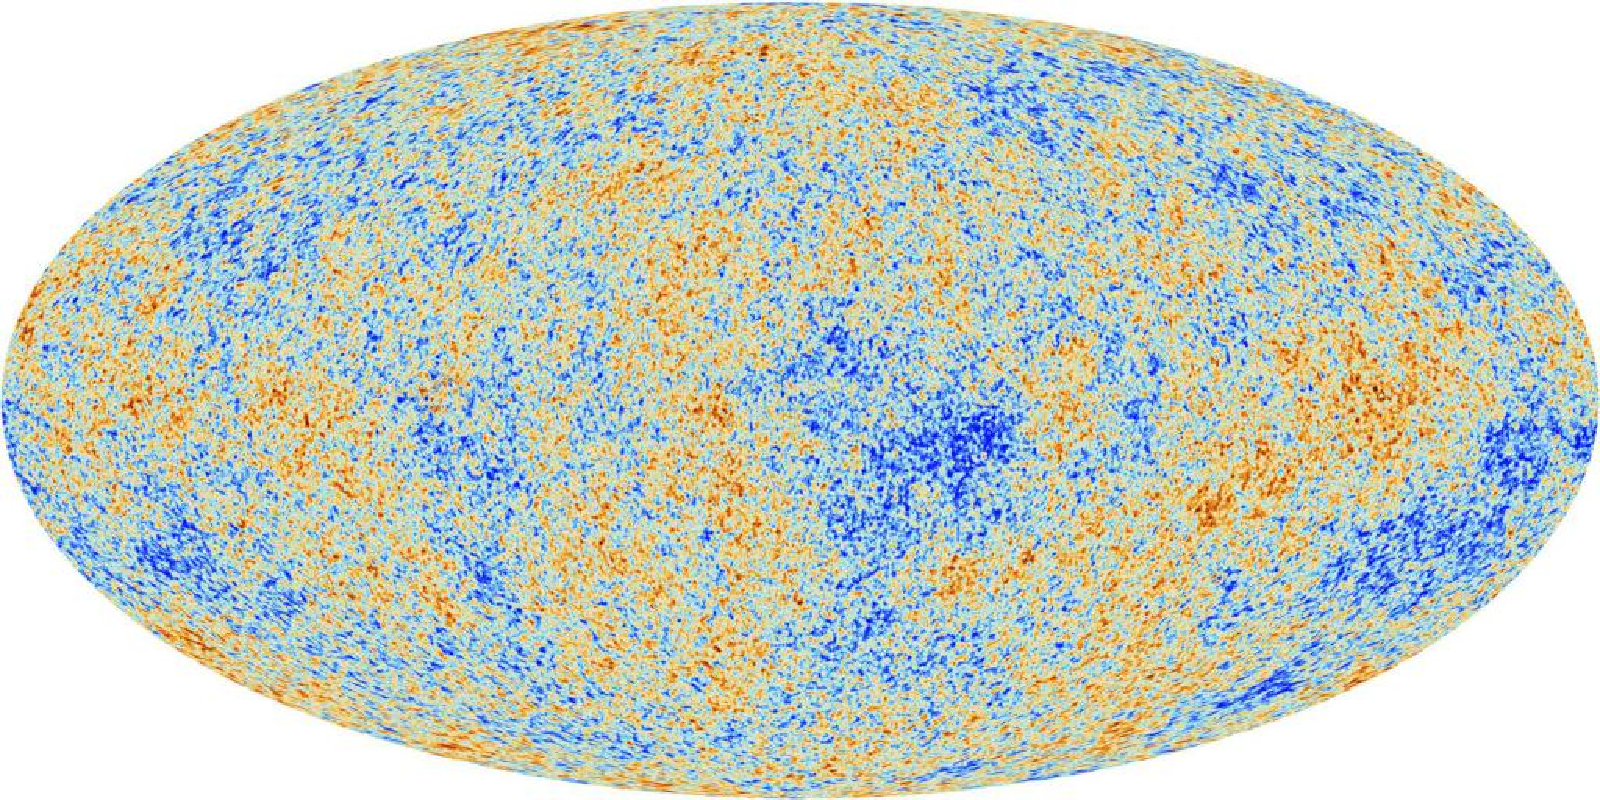
\includegraphics[width=\textwidth]{figs/unit08_CMB.pdf}\end{center}

The final figure below illustrates such a fit of CMB data to the Planck spectrum, using measurements taken by the Cosmic Background Explorer (COBE) satellite and \href{https://doi.org/10.1086/185717}{published in 1990}.
(This version of the figure is adapted from that publication, and copied from Schroeder's \textit{Introduction to Thermal Physics}.)
The squares are the measured data, and their size represents a cautious estimate of uncertainties.
They are plotted with the frequency $f = \om / (2\pi)$ on the horizontal axis, with $f \approx 3\times 10^{-11}~\text{s}^{-1}$ corresponding to a low-energy wavelength $\la = c / f \approx 1$~mm, roughly $1000$ times longer than the wavelengths of visible light.
The solid line is a fit to the data that produces $T_{\text{CMB}} = 2.735 \pm 0.060$~K.
While more recent satellites have increased the precision with which we know $T_{\text{CMB}}$, this first result was awarded the 2006 Nobel Prize in Physics.

\begin{center}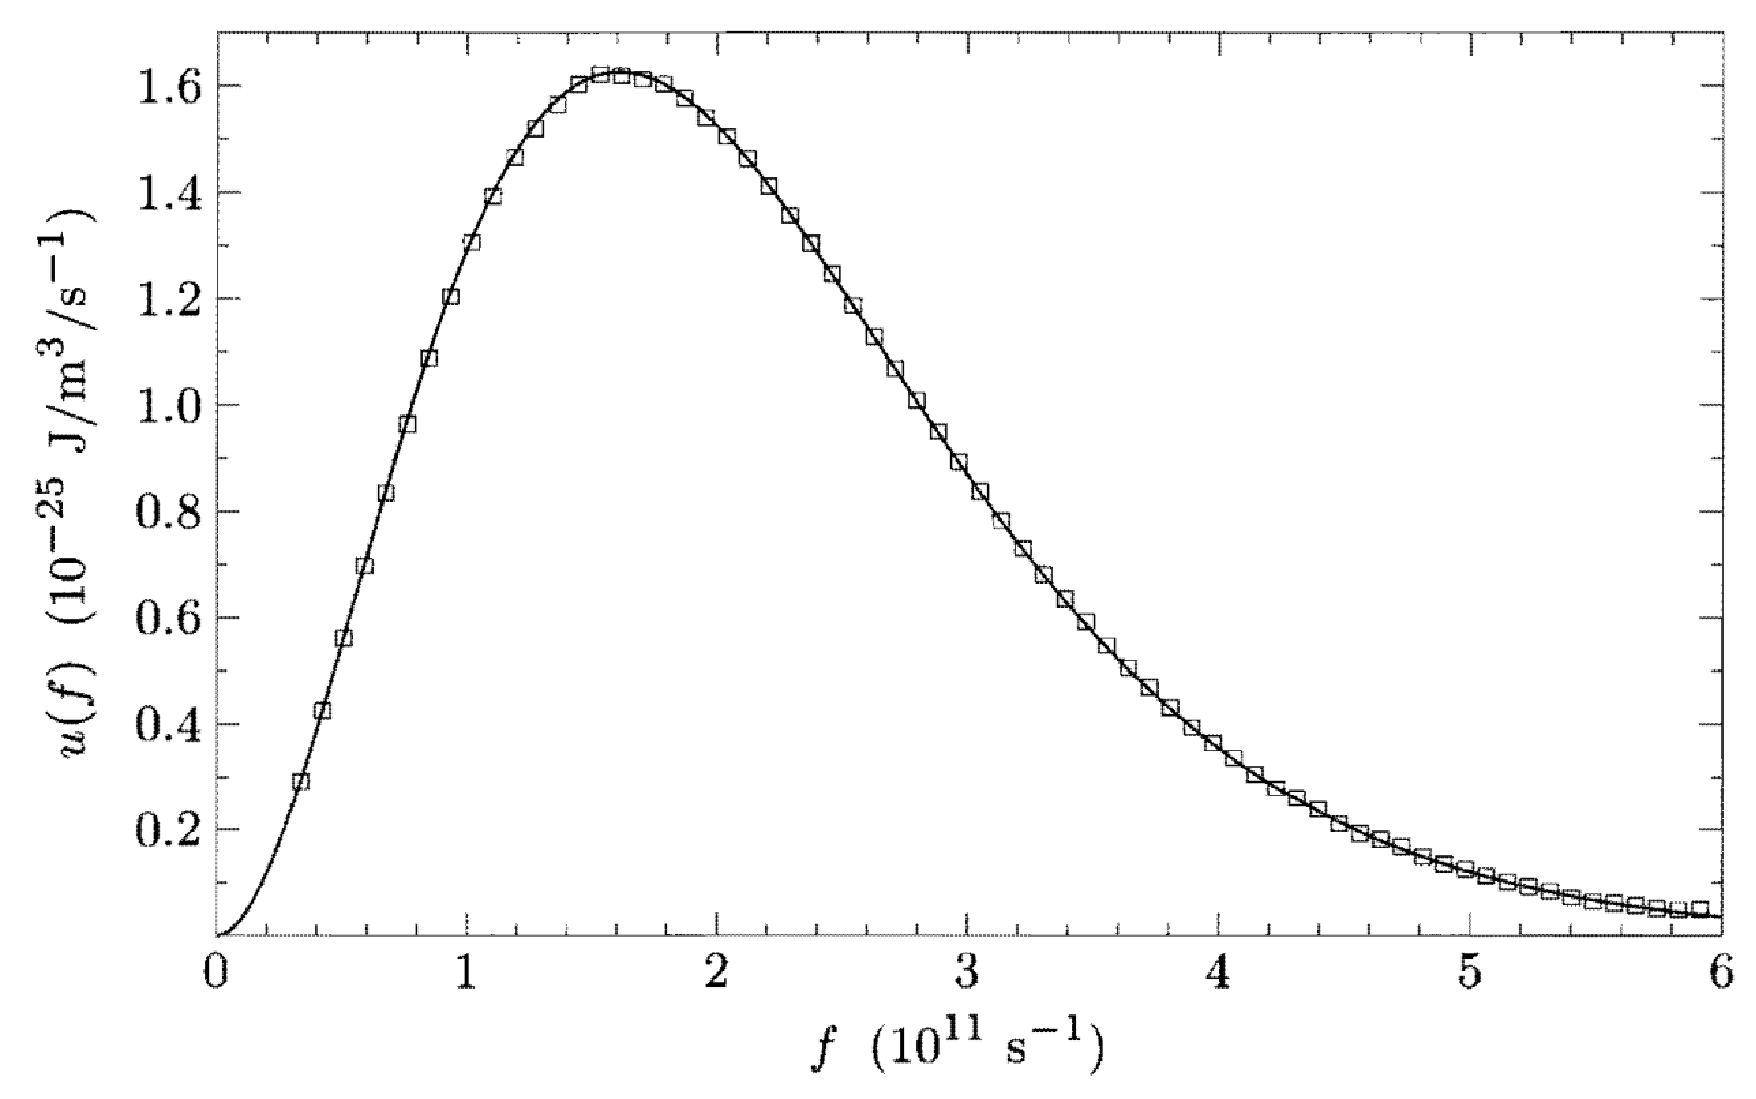
\includegraphics[width=\textwidth]{figs/unit08_COBE.pdf}\end{center}

\begin{shaded}
  Even though we derived the Planck spectrum by assuming an ideal gas of non-interacting photons, we see that it provides an excellent mathematical model for real physical systems, stretching from the hottest to the coldest places in the universe.
\end{shaded}
% ------------------------------------------------------------------



% ------------------------------------------------------------------
\subsection{\label{sec:photon_eos}Equation of state for the photon gas}
Having looked in some detail at the integrand for the photon gas energy density, \eq{eq:Planck_omega}, let's complete the integration, which involves a famous integral related to the Riemann zeta function:
\begin{equation*}
  I_4 = \int_0^{\infty} \frac{x^3}{e^x - 1} dx = \Gamma(4) \zeta(4) = \frac{\pi^4}{15}.
\end{equation*}
Using this result, what is the average energy density for an ideal photon gas?
\begin{mdframed}
  $\displaystyle \frac{\vev{E}_{\text{ph}}}{V} = \frac{\hbar}{c^3 \pi^2} \int_0^{\infty} \frac{\om^3}{e^{\be \hbar \om} - 1} \; d\om = $ \\[120 pt] % WARNING: ADJUSTED SIZE BY HAND TO FILL REMAINDER OF PAGE
\end{mdframed}

You should find a result proportional to $T^4$, which appears significantly more complicated than \eq{eq:ideal_energy} for the energy of an $N$-particle non-relativistic ideal gas in the canonical ensemble.
This is related to the fluctuating particle number now that we are working in the grand-canonical ensemble.
It's possible to simplify the current situation by computing the average photon number from \eq{eq:N_grand},
\begin{equation*}
  \vev{N}_{\text{ph}} = -\left. \pderiv{}{\mu} \Phi_{\text{ph}}\right|_{\mu = 0} = -\left. \frac{VT}{c^3 \pi^2} \int_0^{\infty} d\om \; \om^2 \pderiv{}{\mu} \log\left[1 - e^{-\be \hbar \om} e^{\be \mu}\right] \right|_{\mu = 0},
\end{equation*}
recalling $\mu = 0$ for photon gases.
The calculation is quite similar to that for the average internal energy density, now involving the integral
\begin{equation*}
  I_3 = \int_0^{\infty} \frac{x^2}{e^x - 1} dx = \Gamma(3) \zeta(3) = 2\zeta(3).
\end{equation*}
Using this result, what is the average particle number density ideal photon gas?
\begin{mdframed}
  $\displaystyle \frac{\vev{N}_{\text{ph}}}{V} = -\left. \frac{T}{c^3 \pi^2} \int_0^{\infty} d\om \; \om^2 \pderiv{}{\mu} \log\left[1 - e^{-\be \hbar \om} e^{\be \mu}\right] \right|_{\mu = 0} = $ \\[120 pt]
\end{mdframed}

You should find a result proportional to $T^3 \propto \vev{E}_{\text{ph}} / T$, so that
\begin{equation}
  \label{eq:photon_gas_energy}
  \vev{E}_{\text{ph}} = \frac{\pi^2}{15 \hbar^3 c^3} VT^4 = \frac{\pi^4}{30\zeta(3)} \vev{N}_{\text{ph}} T.
\end{equation}
The functional form is the same as \eq{eq:ideal_energy}, with a larger numerical factor
\begin{equation*}
  \frac{\pi^4}{30\zeta(3)} = \frac{\Gamma(4) \zeta(4)}{\Gamma(3) \zeta(3)} \approx 2.7
\end{equation*}
compared to the $\frac{3}{2}$ for the classical non-relativistic case.

To get the rest of the way to the equation of state for the photon gas, we need to compute the \textit{radiation pressure}
\begin{equation*}
  P_{\text{ph}} = -\left. \pderiv{}{V} \vev{E}_{\text{ph}} \right|_{S_{\text{ph}}},
\end{equation*}
which requires first figuring out the condition of constant entropy $S_{\text{ph}}$ for a photon gas.
From \eq{eq:grand_relation} with $\mu = 0$, we have
\begin{equation*}
  S_{\text{ph}} = \frac{\vev{E}_{\text{ph}} - \Phi_{\text{ph}}}{T}.
\end{equation*}
Looking back to \eq{eq:photon_grand} for the grand-canonical potential, we see
\begin{equation*}
  \frac{\Phi_{\text{ph}}}{T} = \frac{V}{c^3 \pi^2} \int_0^{\infty} d\om \; \om^2 \log\left[1 - e^{-\be \hbar \om}\right] = \frac{VT^3}{\hbar^3 c^3 \pi^2} \int_0^{\infty} dx \; x^2 \log\left[1 - e^{-x}\right],
\end{equation*}
changing variables to $x = \be \hbar \om = \hbar \om / T$.
The final factor in this expression is yet another delightful integral,
\begin{equation*}
  \int_0^{\infty} dx \; x^2 \log\left[1 - e^{-x}\right] = -2\zeta(4) = -\frac{\pi^4}{45}.
\end{equation*}
Since this gives us $S \propto VT^3$, we can conclude that the condition of constant entropy for a photon gas is $V T^3 = \mbox{constant}$, in contrast to the $V T^{3/2}$ dependence of \eq{eq:ideal_entropy} for classical non-relativistic particles.

At this point it is straightforward to take the derivative of the average internal energy if we express the constant-entropy condition as $T = b V^{-1 / 3}$, with $b$ a constant:
\begin{mdframed}
  $\displaystyle P_{\text{ph}} = -\left. \pderiv{}{V} \vev{E}_{\text{ph}} \right|_{S_{\text{ph}}} = -\left. \pderiv{}{V} \frac{\pi^2}{15 \hbar^3 c^3} V T^4 \right|_{S_{\text{ph}}} = $ \\[120 pt]
\end{mdframed}
For the resulting equation of state for the photon gas, you should find
\begin{equation}
  P_{\text{ph}} V = \frac{1}{3} \vev{E}_{\text{ph}} = \frac{\pi^4}{90\zeta(3)} \vev{N}_{\text{ph}} T.
\end{equation}
The functional form is the same as the (classical, non-relativistic) ideal gas law, with just an additional numerical factor of
\begin{equation*}
  \frac{\pi^4}{90\zeta(3)} = \frac{\zeta(4)}{\zeta(3)}. % TODO: Approximately 0.9...
\end{equation*}
% ------------------------------------------------------------------



% ------------------------------------------------------------------
\newpage % WARNING: FORMATTING BY HAND
\subsection{\label{sec:fermi_nonrel}Non-relativistic ideal fermion gas}
For the remainder of this unit we will turn our attention to applying the grand-canonical ensemble to investigate ideal gases of non-interacting fermions.
We again take the approach of quantum statistics, defining micro-states by summing over the possible occupation numbers $n_{\ell}$ for each energy level $\cE_{\ell}$ with (possibly not unique) energy $E_{\ell}$.
In contrast to the bosonic case considered above, the only possible occupation numbers are now $n_{\ell} = 0$ and $1$, since the Pauli exclusion principle prevents multiple identical fermions from occupying the same energy level.

In \secref{sec:fermi} we derived the grand-canonical partition function (\eq{eq:partfunc_FD}) that defines quantum Fermi--Dirac statistics for such systems of non-interacting fermions,
\begin{equation*}
  \ZFD(\be, \mu) = \prod_{\ell = 0}^{\cL} \left[1 + e^{-\be (E_{\ell} - \mu)}\right],
\end{equation*}
in terms of the inverse temperature $\be = 1 / T$ and chemical potential $\mu$.
Recall that it is possible for systems of fermions to have any value for the chemical potential, either positive or negative, in contrast to the systems of bosons we considered above.
From the corresponding grand-canonical potential,
\begin{equation*}
  \Phi_{\text{FD}} = -T\log \ZFD = -T \sum_{\ell = 0}^{\cL} \log\left[1 + e^{-\be (E_{\ell} - \mu)}\right]
\end{equation*}
we can determine the large-scale properties of the system, including its average internal energy $\vev{E}$, average particle number $\vev{N}$, entropy $S$, and pressure $P$, along with the equation of state relating these quantities.

Concrete calculations require specifying the energy levels of the particles that compose the gas, including the degeneracies of any distinct energy levels $\left\{\cE_m, \cE_n\right\}$, $m \neq n$, with the same energy $E_m = E_n$.
In this section we'll begin by considering non-relativistic particles, expanding on our review of such systems in \secref{sec:photon}.
In a volume $V = L^3$, the energy levels are defined by the non-zero quantized energies
\begin{align*}
  E(k) & = \eps \left(k_x^2 + k_y^2 + k_z^2\right) \qquad &
  \eps & \equiv \frac{\hbar^2 \pi^2}{2mL^2} \qquad &
  k_{x, y, z} & = 1, 2, \cdots.
\end{align*}
In addition to the usual degeneracies coming from permutations of $(k_x, k_y, k_z)$ that we have already analyzed, for each distinct $\vec k$ typical fermions such as electrons have two degenerate energy levels with the same energy $E(k)$.
This arises from a quantum property called \textit{spin}, rather than the two polarizations for photons discussed in \secref{sec:photon}: `spin-up' and `spin-down' electrons with the same momenta and energies occupy distinct, degenerate energy levels.
This property of spin is related to the spin--statistics theorem mentioned in \secref{sec:spin}, and is another topic we can discuss further in a tutorial if there is interest.
For our statistical physics purposes it will suffice simply to incorporate this information into our ansatz as input.

The grand-canonical potential for an ideal gas of non-relativistic fermions is therefore
\begin{equation*}
  \Phi_{\text{f}} = -T \sum_{\ell = 0}^{\cL} \log\left[1 + e^{-\be (E_{\ell} - \mu)}\right] = -2T \sum_{\vec k} \log\left[1 + \exp\left(-\frac{\hbar^2 \pi^2 k^2}{2mL^2 T} + \frac{\mu}{T}\right)\right].
\end{equation*}
We can again proceed by considering the gas in a large volume and approximating the sum over discrete integer $k_{x, y, z}$ by integrals over continuous real $\khat_{x, y, z}$:
\begin{equation*}
  \Phi_{\text{f}} \approx -2T \int d\khat_x \; d\khat_y \; d\khat_z \; \log\left[1 + \exp\left(-\frac{\hbar^2 \pi^2 \khat^2}{2mL^2 T} + \frac{\mu}{T}\right)\right].
\end{equation*}
Converting to spherical coordinates and carrying out the angular integrations over the $\frac{\pi}{2}$ solid angle of the octant of the sphere with $k_{x, y, z} > 0$, we have
\begin{equation*}
  \Phi_{\text{f}} \approx -\pi T \int_0^{\infty} d\khat \; \khat^2 \log\left[1 + \exp\left(-\frac{\hbar^2 \pi^2 \khat^2}{2mL^2 T} + \frac{\mu}{T}\right)\right].
\end{equation*}
In the same spirit as the change of variables we carried out to integrate over photon frequencies $\om = \Eph / \hbar$, we will now change variables to integrate over the fermion energy $E = \displaystyle \frac{\hbar^2 \pi^2}{2mL^2}\khat^2$:
\begin{mdframed}
  $\displaystyle \Phi_{\text{f}} = $ \\[120 pt]
\end{mdframed}

As for the case of a photon gas, \eq{eq:photon_grand}, you should find $\Phi_{\text{f}} \propto VT$.
It will be convenient to keep this grand-canonical potential in the form of an integral over the energy $E$, which we will evaluate after taking appropriate derivatives to determine the thermodynamics and equation of state for non-relativistic fermions.
% ------------------------------------------------------------------



% ------------------------------------------------------------------
\subsection{\label{sec:fermi_lowT}Low-temperature equation of state}
In contrast to the photon gas, we need to retain the chemical potential in our analyses of non-relativistic fermions, which makes these calculations more complicated.
To achieve a different simplification, we can focus on the low-temperature regime where we expect quantum Fermi--Dirac statistics to differ significantly from the classical case we considered back in \secref{sec:regulate}.
As we saw in \secref{sec:quantum_classical}, it is only at high temperatures, with large negative chemical potential, that the classical approach provides a good approximation to the true quantum physics.

To see how low temperatures simplify the analysis of the non-relativistic fermion gas, it will prove profitable to first analyze the average particle number
\begin{equation*}
  \vev{N}_{\text{f}} = -\pderiv{}{\mu} \Phi_{\text{f}},
\end{equation*}
using the grand-canonical potential we computed above.
In analogy to the Planck spectrum we derived for the photon gas in \secref{sec:planck}, we first express the average particle number density as an integral over energies,
\begin{equation}
  \label{eq:N_fermi}
  \frac{\vev{N}_{\text{f}}}{V} = \frac{\sqrt{2m^3}}{\pi^2 \hbar^3} \int_0^{\infty} F(E) \sqrt{E} \; dE,
\end{equation}
where the function $F(E)$ is known as the Fermi function.
In contrast to the Planck spectrum, some constant factors are kept separate from $F(E)$, so that it more closely resembles the average occupation numbers $\vev{n_{\ell}}$ we computed in \secref{sec:quantum_classical}:
\begin{mdframed}
  $\displaystyle \frac{\vev{N}_{\text{f}}}{V} = -\pderiv{}{\mu} \frac{\Phi_{\text{f}}}{V} = $ \\[120 pt]
\end{mdframed}

As usual in the grand-canonical approach, the average particle number density and Fermi function depend on both the inverse temperature \be and the chemical potential $\mu$.
Expressing $F(E)$ in terms of the dimensionless ratios $E / \mu$ and $T / \mu$,
\begin{equation*}
  F(E) = \frac{1}{\exp\left[\frac{E - \mu}{T}\right] + 1} = \frac{1}{\exp\left[\frac{\mu}{T}\left(\frac{E}{\mu} - 1\right)\right] + 1} = \frac{1}{\left(\exp\left[\frac{E}{\mu} - 1\right]\right)^{\mu / T} + 1},
\end{equation*}
we can highlight the two main features of the figure below, which plots the Fermi function against $E / \mu$ for various temperatures $T / \mu$.
Here we assume a positive chemical potential, $\mu > 0$, which we will soon show is required for low-temperature non-relativistic fermion gases.

First, we can see that the point $E = \mu$, where $F(E) = 1 / 2$ for any non-zero temperature, is a threshold at which the behaviour of the Fermi function changes.
For larger energies $E > \mu$, the exponential factor $\exp\left[\frac{E}{\mu} - 1\right] > 1$ and drives $F(E) \to 0$ as the energy increases.
For smaller energies $E < \mu$, the exponential factor $\exp\left[\frac{E}{\mu} - 1\right] < 1$ and vanishes as the energy decreases, leaving $F(E) \to 1$.
These two asymptotic limits reflect the possible energy level occupation numbers for fermions, $n_{\ell} = 0$ and $1$.
Second, smaller temperatures cause much more rapid approach to these two limits, with the exponential factor either enhanced (if $E > \mu$) or suppressed (if $E < \mu$) by a power $\mu / T \gg 1$.

\begin{center}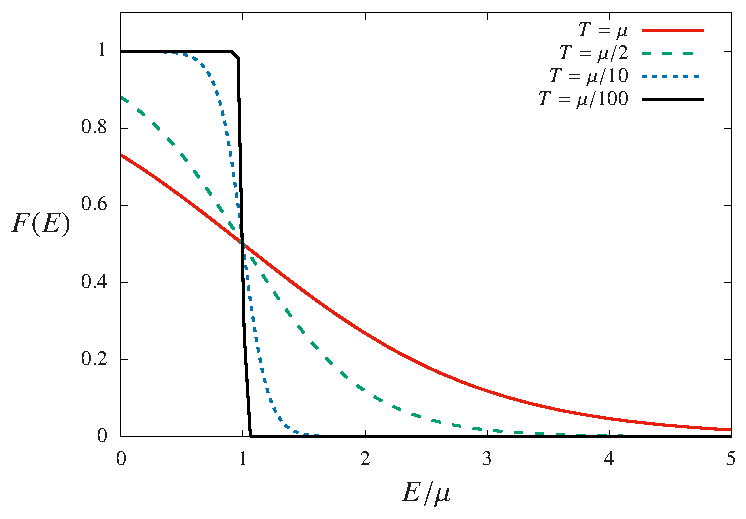
\includegraphics[width=\textwidth]{figs/unit08_dist.pdf}\end{center}

Therefore, for small temperatures $T \ll \mu$, we can simplify our calculations by approximating the Fermi function as a step function,
\begin{equation}
  \label{eq:Fermi_step}
  F(E) \approx \left\{\begin{array}{l}1 \qquad \mbox{for } \ E < \mu \\
                                      0 \qquad \mbox{otherwise}\end{array}\right. .
\end{equation}
Using this approximation, what is the resulting average particle number density?
\begin{mdframed}
  $\displaystyle \frac{\vev{N}_{\text{f}}}{V} = \frac{\sqrt{2m^3}}{\pi^2 \hbar^3} \int_0^{\infty} F(E) \sqrt{E} \; dE = $ \\[100 pt]
\end{mdframed}

You should find a result proportional to $\mu^{3 / 2}$ but independent of $T$.
The temperature independence turns out to be the leading-order behaviour of a more general result that can be organized in powers of the small temperature, $T / \mu \ll 1$, through a method known as the \textit{Sommerfeld expansion} (named after \href{https://en.wikipedia.org/wiki/Arnold_Sommerfeld}{Arnold Sommerfeld}).
The $\mu^{3 / 2}$ dependence on the chemical potential is something we could have predicted before doing the explicit calculation.
This is because the step function in \eq{eq:Fermi_step} corresponds to a single fermion occupying each and every energy level with $E_{\ell} < \mu$, while all energy levels with $E_{\ell} > \mu$ are unoccupied.
Since $E(k) \propto k^2$, summing over all $k_{x, y, z}$ for which $E(k) < \mu$ corresponds to computing (a portion of) the volume of a sphere of radius $r_k = \sqrt{\mu}$.
This volume is proportional to $r_k^3 = \mu^{3 / 2}$, in agreement with our result above.
If we invert that result, we obtain the so-called \textbf{Fermi energy} as a function of the average particle number density, % TODO: Remove `so-called'...
\begin{equation}
  \label{eq:Fermi_energy}
  E_F = \mu = \frac{\hbar^2}{2m}\left(\frac{3\pi^2 \vev{N}_{\text{f}}}{V}\right)^{2 / 3}.
\end{equation}
Like the step-function approximation to the Fermi function, this equality between the Fermi energy and the chemical potential is only exact at zero temperature, with $T > 0$ introducing small corrections that take some work to compute. % TODO: Could introduce Fermi energy as radius of energy sphere into which all N particles could be packed...

Now we can consider the average energy density of the non-relativistic fermion gas at low temperatures.
Rather than taking another derivative of the grand-canonical potential, we can note from \eq{eq:total_energy_levels} and from our work on the photon gas in \secref{sec:photon_eos} that
\begin{equation}
  \frac{\vev{E}_{\text{f}}}{V} = \frac{\sqrt{2m^3}}{\pi^2 \hbar^3} \int_0^{\infty} E \; F(E) \sqrt{E} \; dE.
\end{equation}
That is, instead of simply counting the number of fermions in the system, we need to add up their energies, introducing an extra factor of $E$ compared to \eq{eq:N_fermi}.
Still using the low-temperature step-function approximation for the Fermi function in \eq{eq:Fermi_step}, what is the average energy density?
\begin{mdframed}
  $\displaystyle \frac{\vev{E}_{\text{f}}}{V} = \frac{\sqrt{2m^3}}{\pi^2 \hbar^3} \int_0^{\infty} F(E) \; E^{3 / 2} \; dE = $ \\[100 pt]
\end{mdframed}
You should find
\begin{equation}
  \label{eq:fermi_E_N}
  \vev{E}_{\text{f}} = \frac{3}{5} \mu \vev{N}_{\text{f}},
\end{equation}
which means that the average energy of each fermion in a low-temperature ideal gas, $\vev{E}_{\text{f}} / \vev{N}_{\text{f}}$, is three-fifths of the Fermi energy $E_F = \mu$.

\begin{shaded}
  In particular, because \eq{eq:fermi_E_N} is independent of the temperature, we find that non-interacting quantum fermions retain a positive energy even as the temperature approaches absolute zero, $T \to 0$.
\end{shaded}

This can be understood by recalling that the lowest-energy pair of degenerate energy levels can each only hold a single fermion, forcing any additional fermions to `fill' energy levels with larger energies $E_{\ell} > 0$, up to the Fermi energy set by the chemical potential.
This is a stark contrast to the $\vev{E} = \frac{3}{2} N T$ we found for classical ideal gases in the canonical ensemble in \eq{eq:ideal_energy}, as well as the $\vev{E}_{\text{ph}} \approx 2.7 \vev{N}_{\text{ph}} T \propto T^4$ we more recently computed in \eq{eq:photon_gas_energy} for a grand-canonical quantum gas of photons.
In both of those cases the average energy vanishes in the zero-temperature limit.
This is because all the particles in those classical and bosonic systems are able to occupy the lowest energy level at low temperatures, with only exponentially small probabilities $\propto e^{-E_{\ell}/ T}$ for particles to occupy any energy levels with $E_{\ell} > E_0$.

This picture of fermions filling energy levels up to the Fermi energy also clarifies why the chemical potential for a fermion gas must be positive at low temperatures.
Recalling \eq{eq:mu_E} for the chemical potential,
\begin{equation*}
  \mu = \left.\pderiv{E}{N}\right|_{S, V},
\end{equation*}
which we derived from the generalized thermodynamic identity in \secref{sec:grand_pot}, we can consider what happens when we increase the number of particles in a zero-temperature fermion gas.
In this limit $T \to 0$, there is only the single quantum micro-state described above, with all energy levels filled below the Fermi energy and empty above the Fermi energy.
Adding particles, $\De N > 0$, doesn't increase the number of accessible micro-states, and therefore doesn't increase the entropy $S_{\text{f}} = -\sum_{i = 1}^M p_i \log p_i = 0$, satisfying the constant-entropy condition required by this equation.
However, this does necessarily increase the energy, because the added particles must fill the first available energy levels, just above the Fermi energy. % TODO: Could remind of continuous approximation used to change from sums to integrals above...
That is, $\De E = E_F \De N > 0$, and we find $\mu = E_F > E_0 \geq 0$ as claimed earlier in this section.
It is an interesting but lengthy exercise (discussed in the supplement below) to show that the chemical potential becomes negative as the temperature increases and we approach the classical limit.

To get the rest of the way to the low-temperature equation of state for ideal gases of non-relativistic fermions, we need to compute the pressure
\begin{equation*}
  P_{\text{f}} = -\left. \pderiv{}{V} \vev{E}_{\text{f}} \right|_{N, S_{\text{f}}}.
\end{equation*}
As we just discussed, the single accessible micro-state for $T \to 0$ automatically satisfies the condition of constant entropy, $S_{\text{f}} = 0$.
Applying \eq{eq:Fermi_energy} relating the chemical potential to the average particle number density, we have
\begin{equation*}
  \vev{E}_{\text{f}} = \frac{3}{5} \mu \vev{N}_{\text{f}} = \frac{3}{5} \left(\frac{\hbar^2}{2m}\right) \left(\frac{3\pi^2}{V}\right)^{2 / 3} \vev{N}_{\text{f}}^{5 / 3}.
\end{equation*}
This is all we need to determine the pressure, which we can relate to the energy density, the Fermi energy $E_F = \mu$ and the particle number density:
\begin{mdframed}
  $\displaystyle P_{\text{f}} = -\pderiv{}{V} \left[\frac{3}{5} \left(\frac{\hbar^2}{2m}\right) \left(\frac{3\pi^2}{V}\right)^{2 / 3} \vev{N}_{\text{f}}^{5 / 3}\right] = $ \\[100 pt]
\end{mdframed}
In particular, we can see that the pressure (like the energy) remains positive even as the temperature approaches absolute zero, with
\begin{equation}
  \label{eq:degen_pressure}
  P_{\text{f}} = \left(3\pi^2\right)^{2 / 3} \frac{\hbar^2}{5m} \rho_{\text{f}}^{5 / 3},
\end{equation}
where we define the density $\rho_{\text{f}} = \vev{N}_{\text{f}} / V$.
This positive pressure in the zero-temperature limit is not due to any direct force between the fermions, which remain non-interacting in this ideal gas.
Instead, it is a purely quantum effect resulting from the Pauli exclusion principle.

As we saw earlier in this section, the temperature independence of the pressure $P_{\text{f}}$ is due to approximating the low-temperature Fermi function as a step function in \eq{eq:Fermi_step}, and systematic corrections to this approximation can be computed through a Sommerfeld expansion.
Even without getting into such detailed calculations, we know that in the high-temperature classical regime the quantum ideal gas of massive fermions will be well approximated by the classical ideal gas we considered in \secref{sec:ideal_gas}, with equation of state
\begin{equation}
  PV = NT \qquad \Lra \qquad P = \frac{N}{V} T = \rho T.
\end{equation}
In words, at high temperatures the pressure depends linearly on the temperature, with the slope corresponding to the density $\rho$.
The plot below (produced by \href{https://github.com/daschaich/MATH327_2022/blob/master/lecture_notes/figs/unit08_pressure.py}{this Python code}) shows how the pressure changes from a positive constant as $T \to 0$ to this linear behaviour at higher temperatures. \\[-24 pt]
\begin{center}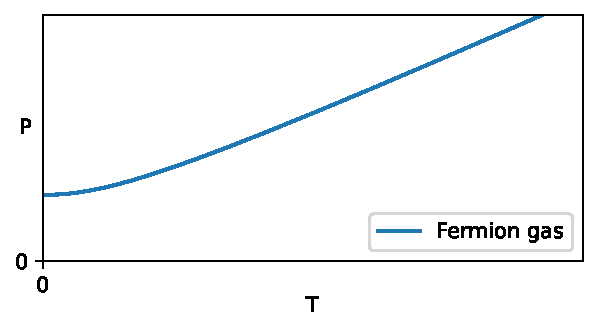
\includegraphics[width=0.7\textwidth]{figs/unit08_pressure.pdf}\end{center} % WARNING: ADJUSTED SIZE BY HAND TO FILL REMAINDER OF PAGE
% ------------------------------------------------------------------



% ------------------------------------------------------------------
\subsection{Type-{\textrm I}a supernovas}
The positive pressure that remains for a fermion gas even at zero temperature, \eq{eq:degen_pressure}, is known as the \textit{degeneracy pressure}.
(This use of the word `degeneracy' is unrelated to its other use describing multiple energy levels with the same value of the energy.)
The degeneracy pressure plays a key role in a certain type of supernova explosions of stars --- a famous astrophysical phenomenon.

To begin considering this topic, we'll remark that the temperature doesn't need to be exactly zero in order for the degeneracy pressure to be significant.
The temperature just needs to be small compared to the Fermi energy, $T \ll E_F$.
From \eq{eq:Fermi_energy} we can see that $E_F \propto \rho_{\text{f}}^{2 / 3}$ increases for larger densities $\rho_{\text{f}} = \vev{N}_{\text{f}} / V$.
Not surprisingly, the densities of stars can be very large indeed, due to the enormous amount of matter that is being squeezed together by gravitational attraction.
Everyday matter has densities around $10^{28}$--$10^{29}$ atoms per cubic metre (roughly Avogadro's number per cubic centimetre), which corresponds to Fermi energies $E_F \sim 10^4$~K, very large compared to everyday temperatures. % 2--10 eV with eV~10^4 K being the Boltzmann constant
Fermi energies for particularly dense stars known as \textit{white dwarfs} are a hundred thousand times larger still, $E_F \sim 10^9$~K, with densities around $10^{35}$--$10^{36}$ atoms per cubic metre roughly equivalent to a mass density of one tonne per cubic centimetre. % ~10^(−27) kg per amu times 10^(36) / (10^2)^3 particles gives ~1000 kg per cc
This is around a million times more dense than our sun --- while white dwarf stars have a mass similar to our sun's $M_{\odot}$, their radius is a hundred times smaller, comparable to the radius of the earth.

White dwarf stars are so dense because they have exhausted the hydrogen and helium `fuel' for the nuclear fusion that generates heat and light --- and therefore radiation pressure --- in stars such as our sun.
For actively `burning' stars, this radiation pressure counteracts the gravitational attraction of the star's enormous mass.
Without nuclear fusion, white dwarfs end up gravitationally compressed into much denser and more compact objects.
The degeneracy pressure, \eq{eq:degen_pressure}, coming from the (fermionic) electrons in the white dwarf is what stabilizes these stars and prevents them from collapsing further into even denser objects such as black holes.

It is remarkable that even under these extreme conditions the electrons in white dwarf stars are well described by the non-interacting ideal fermion gas we analyzed above.
In particular, it is crucial that white dwarfs' Fermi energies are so large, $E_F \sim 10^9$~K.
Even though white dwarfs have burned all their nuclear fuel, their interiors remain quite hot by everyday standards, roughly ten million kelvin ($T \sim 10^7$~K). % 0.3 MeV ~ 10^5 eV with eV~10^4 K being the Boltzmann constant
It is only due to their large densities and Fermi energies that $T \ll E_F$ and white dwarfs can be treated as zero-temperature objects to a good approximation.

So far we haven't encountered supernovas.
In isolation, white dwarfs will happily cool for trillions of years, supported by their degeneracy pressure, until they reach thermal equilibrium with the low-temperature cosmic microwave background radiation we discussed in \secref{sec:planck}.
Things become more interesting for a white dwarf in a binary system with a companion star.
If this companion star is still burning hydrogen or helium through nuclear fusion, it will emit matter that is then captured by the white dwarf, slowly increasing the white dwarf's mass.
Such a binary system is pictured below, in an artist's illustration provided by the \href{https://www.esa.int/ESA_Multimedia/Images/2014/09/Artist_s_impression_of_Type_Ia_supernova}{European Space Agency}.

\begin{center}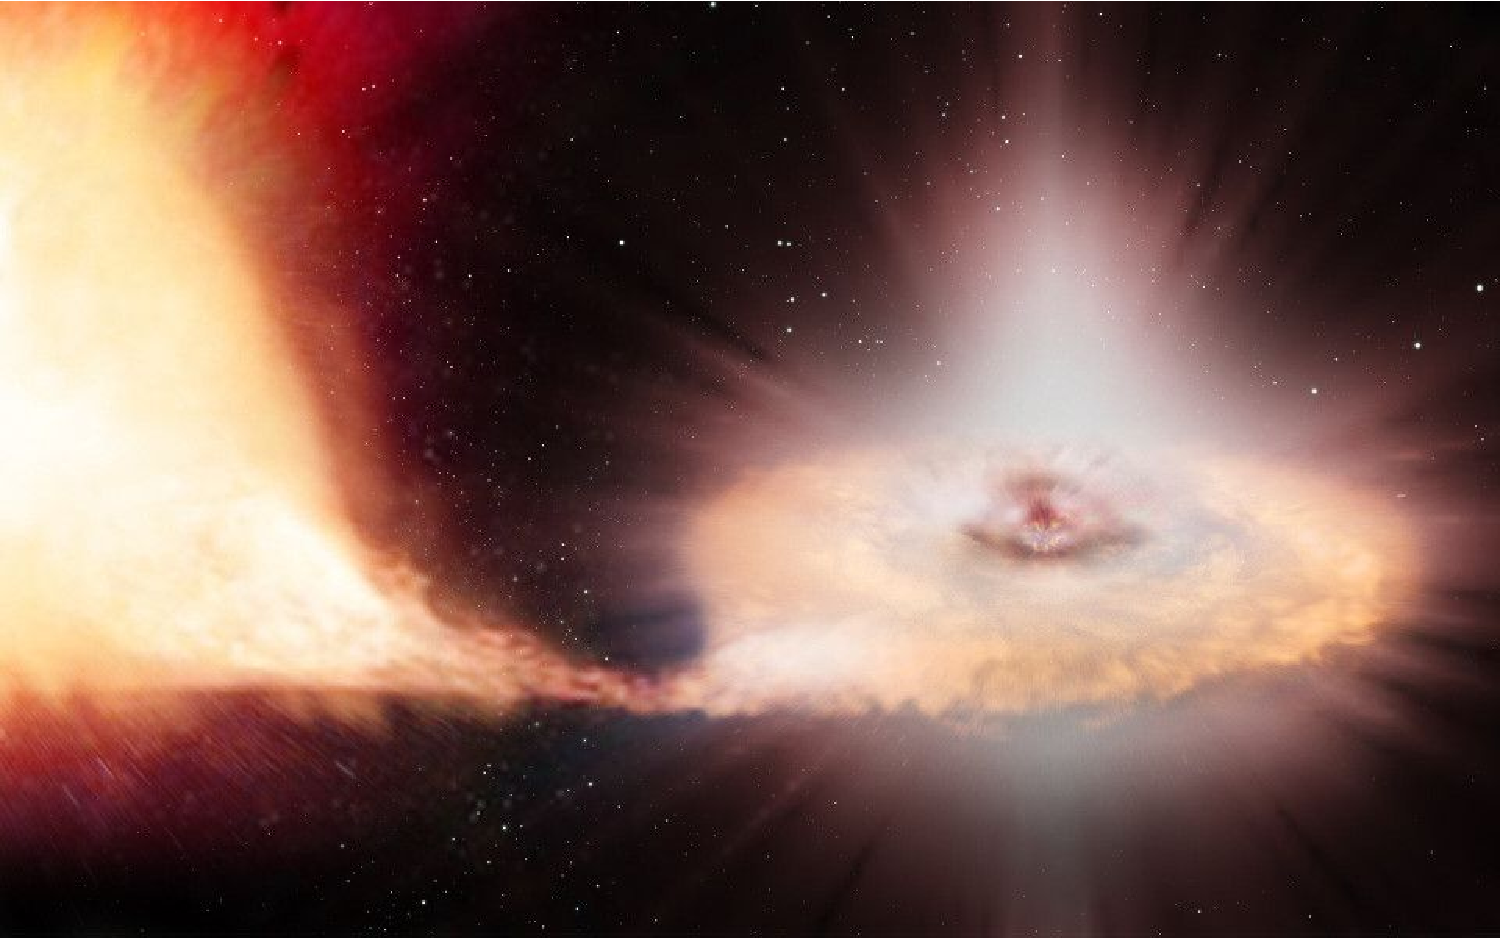
\includegraphics[width=0.8\textwidth]{figs/unit08_nova.pdf}\end{center}

As the white dwarf accumulates the matter emitted by its companion, its mass and its density will steadily increase.
As the mass of the white dwarf approaches a value roughly 40\% larger than the mass of our sun, known as the \textit{Chandrasekhar limit} (named after \href{https://en.wikipedia.org/wiki/Subrahmanyan_Chandrasekhar}{Subrahmanyan Chandrasekhar}), its density becomes large enough for new types of nuclear fusion reactions to occur.
Instead of hydrogen or helium, which the white dwarf has already burned, these new fusion reactions involve carbon and oxygen, which remain present in abundance.
In the space of just a few seconds, these fusion reactions run away, increase the temperature of the white dwarf to billions of kelvin, and blast it apart in a supernova explosion about five billion times brighter than the sun.

For obscure historical reasons, these particular stellar explosions are known as \textit{type-{\textrm I}a} (``one-A'') \textit{supernovas}.
They rely on the degeneracy pressure (\eq{eq:degen_pressure}) of a low-temperature gas of non-interacting fermions, which allows a specific amount of mass to build up before the explosion is triggered.
The specificity of the process results in a great deal of regularity among type-{\textrm I}a supernovas, which is very useful to astronomers.
In particular, these type-{\textrm I}a supernovas play a key role in demonstrating that the expansion of the universe is accelerating (a phenomenon popularly called `dark energy'), which was awarded the 2011 Nobel Prize in Physics.
% ------------------------------------------------------------------



% ------------------------------------------------------------------
\subsection{Relativistic ideal fermion gas}
Although we will discuss them more briefly, gases of relativistic fermions also play important roles in nature.
In fact, by changing units we can see that the white dwarf Fermi energy discussed above, $E_F \sim 10^9~\text{K} \sim 0.3$~MeV is comparable to the $0.511$~MeV rest-energy of electrons, suggesting that relativistic effects may be non-negligible in white dwarfs. % eV~10^4 K is the Boltzmann constant
Such relativistic effects are indeed crucial to the computation of the Chandrasekhar limit mentioned above.

While the full calculations required to analyze massive relativistic particles are beyond the scope of this module, we can take advantage of our earlier analyses of gases of massless photons to briefly consider similar gases of massless fermions.
\textit{Neutrinos} (denoted `$\nu$') are physical examples of fermions whose masses are so small that they can be very well approximated as massless.
In fact, for many years neutrinos were thought to be exactly massless --- the discovery that neutrinos have non-zero masses was awarded the 2015 Nobel Prize in Physics.

In the same way as photons, massless fermions would travel at the speed of light, $c$, and have energies $E = cp$ determined by their angular frequencies,
\begin{equation*}
  E_{\nu} = \hbar \om.
\end{equation*}
In a volume $V = L^3$, these energies are quantized as usual,
\begin{equation*}
  \om = \frac{2\pi c}{\la} = c \frac{\pi}{L} k,
\end{equation*}
where $k^2 = k_x^2 + k_y^2 + k_z^2$ and $k_{x, y, z} > 0$ are positive integers.
Just as for the non-relativistic case considered in \secref{sec:fermi_nonrel}, for each distinct $\vec k$ typical massless fermions, including neutrinos, have two degenerate energy levels with the same energy $E(k)$ but opposite spin.

The computations required to analyze a gas of massless fermions are very similar to the work we recently did for photon gases.
In particular, massless fermions are also easy to create and destroy, and therefore well described by a vanishing chemical potential, $\mu \approx 0$.
Again approximating sums over discrete integer $k_{x, y, z}$ by integrals over continuous real $\khat_{x, y, z}$, and changing variables to integrate over the angular frequency, we end up with the grand-canonical potential
\begin{align}
  \Phi_{\nu} = -\frac{VT}{c^3 \pi^2} \int_0^{\infty} d\om \; \om^2 \log\left[1 + e^{-\be \hbar \om}\right]. \label{eq:neutrino_grand}
\end{align}
The only changes here compared to \eq{eq:photon_grand} for the photon $\Phi_{\text{ph}}$ are a couple of negative signs, precisely as we would expect from comparing the Bose--Einstein and Fermi--Dirac grand-canonical potentials in \secref{sec:quantum_classical}.

Due to these negative signs, when we compute derived quantities by taking derivatives of the potential,
\begin{align*}
  \vev{E}_{\nu} & = \pderiv{}{\be} \left[\be \Phi_{\nu}\right] \qquad &
  \vev{N}_{\nu} & = -\left. \pderiv{}{\mu} \Phi_{\nu}\right|_{\mu = 0},
\end{align*}
we will encounter slightly different but equally enjoyable integrals, % Fermi-Dirac integral involving polylog of -1 related to Dirichlet eta function
\begin{align*}
  \int_0^{\infty} \frac{x^3}{e^x + 1} dx & = \left(1 - \frac{1}{2^3}\right) \Gamma(4) \zeta(4) = \frac{7\pi^4}{120}, \\
  \int_0^{\infty} \frac{x^2}{e^x + 1} dx & = \left(1 - \frac{1}{2^2}\right) \Gamma(3) \zeta(3) = \frac{3}{2} \zeta(3).
\end{align*}
Using these results, what are the average internal energy density and the average particle number density for a gas of massless fermions?
\begin{mdframed}
  $\displaystyle \frac{\vev{E}_{\nu}}{V} = -\frac{1}{c^3 \pi^2} \int_0^{\infty} d\om \; \om^2 \pderiv{}{\be} \log\left[1 + e^{-\be \hbar \om}\right] = $ \\[110 pt]
  $\displaystyle \frac{\vev{N}_{\nu}}{V} = \left. \frac{T}{c^3 \pi^2} \int_0^{\infty} d\om \; \om^2 \pderiv{}{\mu} \log\left[1 + e^{-\be \hbar \om} e^{\be \mu}\right] \right|_{\mu = 0} = $ \\[100 pt]
\end{mdframed}

You should again find $\vev{E}_{\nu} \propto \vev{N}_{\nu} T \propto VT^4$, and by noting that
\begin{equation*}
  \frac{\Phi_{\nu}}{T} = \frac{V}{c^3 \pi^2} \left(\frac{T}{\hbar}\right)^3 \int_0^{\infty} dx \; x^2 \log\left[1 + e^{-x}\right] \propto VT^3,
\end{equation*}
we can see that the entropy $S_{\nu} = \left(E_{\nu} - \Phi_{\nu}\right) / T$ is constant when $V T^3 = \mbox{constant}$.
Applying this, what is the pressure for a gas of massless fermions?
\begin{mdframed}
  $\displaystyle P_{\nu} = -\left. \pderiv{}{V} \vev{E}_{\nu} \right|_{S_{\nu}} = $ \\[100 pt]
\end{mdframed}
You should find yet another equation of state with the usual functional form,
\begin{equation*}
  P_{\nu} V = \frac{1}{3} \vev{E}_{\nu} = \frac{7\pi^4}{540\zeta(3)} \vev{N}_{\nu} T,
\end{equation*}
and just a new numerical factor of
\begin{equation*}
  \frac{7\pi^4}{540\zeta(3)} = \frac{(7/8)\zeta(4)}{(3/4)\zeta(3)}. % TODO: Approximately 1.05...
\end{equation*}
% ------------------------------------------------------------------



% ------------------------------------------------------------------
\subsection{Supplement: Density of states \& Sommerfeld expansion}
In \eq{eq:fermi_E_N} we found that the average internal energy of a non-relativistic fermion gas becomes independent of the temperature in the limit $T \to 0$.
This means that its heat capacity,
\begin{equation*}
  c_v = \left. \pderiv{}{T} \vev{E} \right|_{N,V},
\end{equation*}
vanishes in this limit, which we could also see by considering the fluctuation--dissipation relation $c_v = \be^2 \vev{\left(E - \vev{E}\right)^2}$ with only a single micro-state. % TODO: Again module degeneracies...

To derive the non-trivial heat capacity for a gas with a small but non-zero temperature, we need to move beyond approximating the Fermi function
\begin{equation*}
  F(E) = \frac{1}{e^{\be(E - \mu)} + 1}
\end{equation*}
as a step function, and return to the full \eq{eq:N_fermi} for the average particle number,
\begin{equation}
  \label{eq:number}
  \vev{N}_{\text{f}} = V \frac{\sqrt{2m^3}}{\pi^2 \hbar^3} \int_0^{\infty} F(E) \sqrt{E} \; dE \equiv \int_0^{\infty} g(E) \; F(E) \; dE.
\end{equation}
Here we have defined the \textbf{density of states}
\begin{equation*}
  g(E) \equiv V \frac{\sqrt{2m^3}}{\pi^2 \hbar^3} \sqrt{E} \equiv g_0 \; \sqrt{E}
\end{equation*}
as the number of single-particle energy levels per unit energy.
We can read \eq{eq:number} as saying that the total number of particles is given by integrating over the single-particle energy levels, $g(E)$, times the probability $F(E)$ that each of these energy levels is occupied.

The figures below, from Schroeder's \textit{Introduction to Thermal Physics}, illustrate this integral in the case of $T = 0$ (left) and $T > 0$ (right).
As we have already seen, when $T \to 0$ all energy levels with $E < E_F$ are occupied while all those with $E > E_F$ are unoccupied.
With $T > 0$, there is an exponentially suppressed probability for some energy levels with $E > E_F$ to be occupied.
Because the Fermi energy is set by the number of particles,
\begin{equation*}
  E_F = \frac{\hbar^2}{2m}\left(\frac{3\pi^2 \vev{N}_{\text{f}}}{V}\right)^{2 / 3},
\end{equation*}
having some of these particles occupy energy levels with $E > E_F$ requires that an equal number of energy levels with $E < E_F$ be unoccupied.

\noindent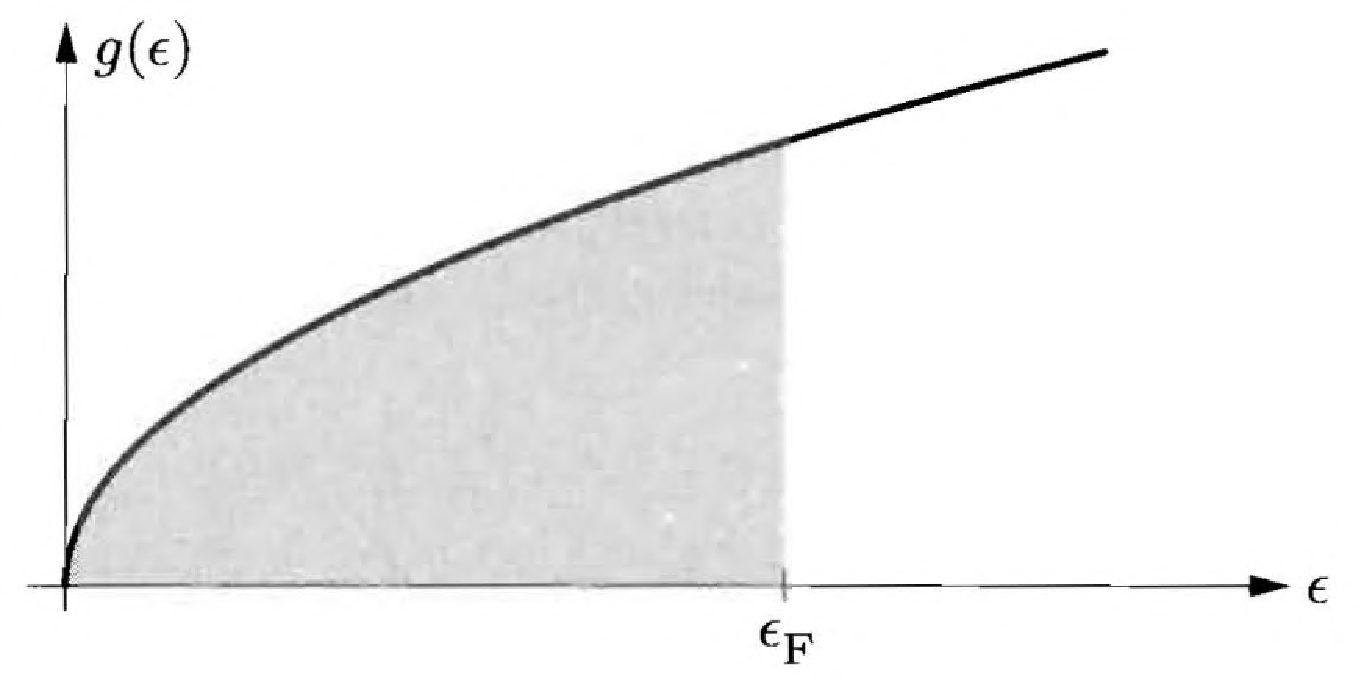
\includegraphics[width=0.45\textwidth]{figs/unit08_zero.pdf}\hfill 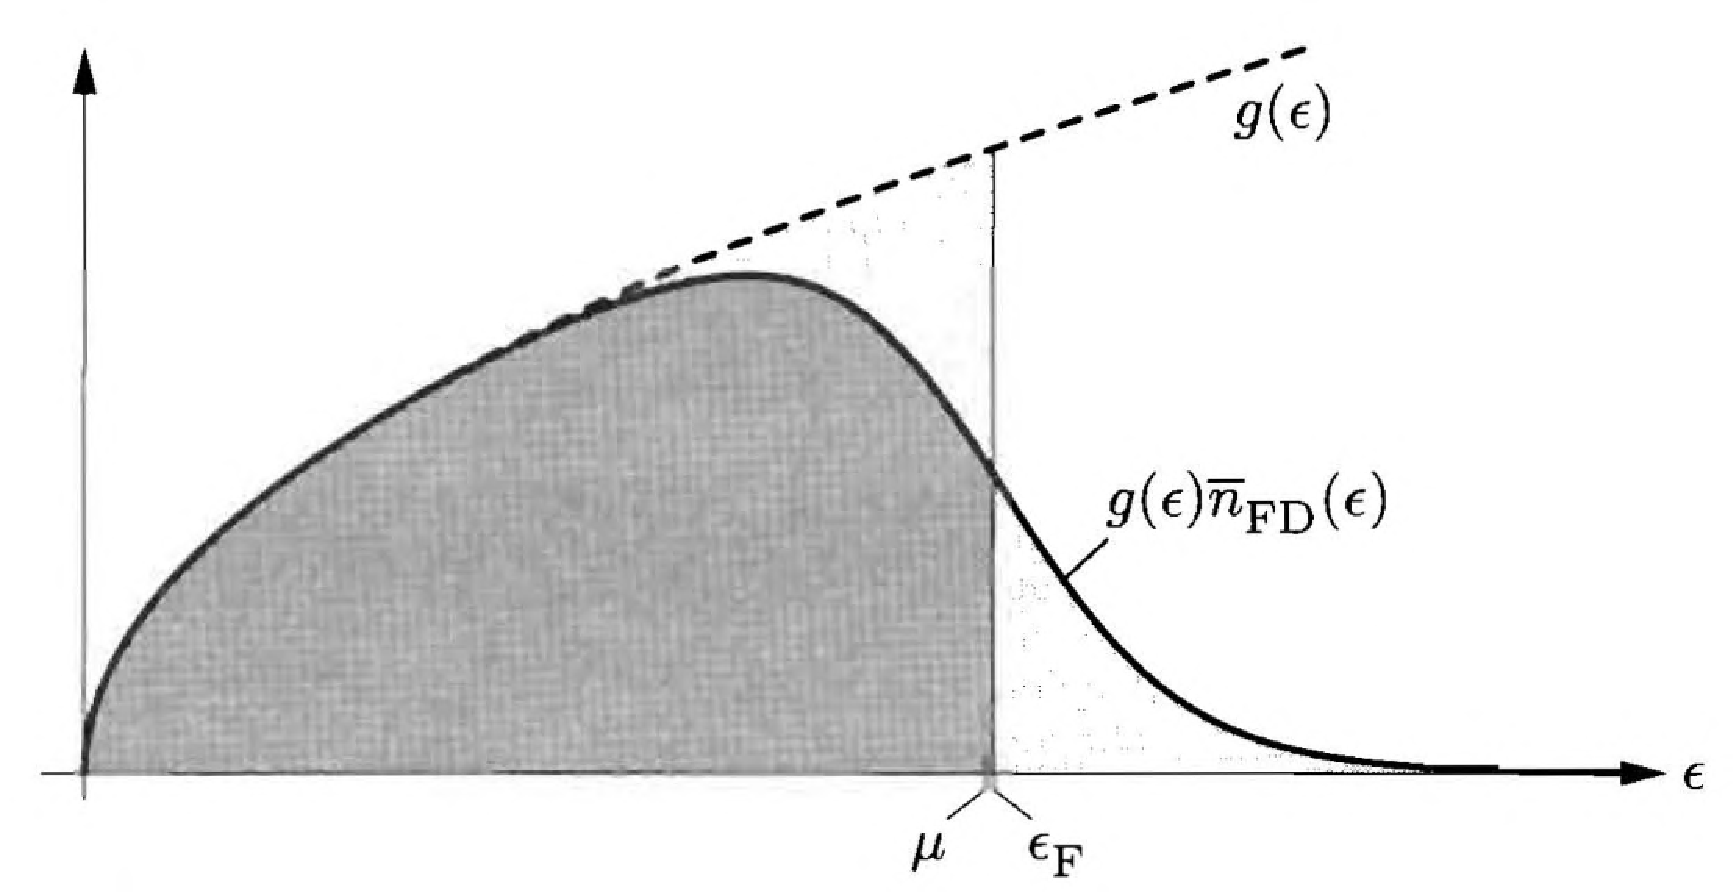
\includegraphics[width=0.45\textwidth]{figs/unit08_nonzero.pdf}

Note that $E = \mu$ is the point where the Fermi function $F(E) = \frac{1}{2}$.
We will see below that $\mu \leq E_F$, as shown in the right figure above, with equality when $T = 0$.

In order to determine the particle number and internal energy, we need to evaluate the integrals
\begin{align}
  \label{eq:DoS_full}
  \vev{N}_{\text{f}} & = g_0 \int_0^{\infty} F(E) \sqrt{E} \; dE \qquad &
  \vev{E}_{\text{f}} & = g_0 \int_0^{\infty} E \; F(E) \sqrt{E} \; dE
\end{align}
without approximating the Fermi function as a step function.
For $T \ll E_F$, we can do this through a \textbf{Sommerfeld expansion}.
Let's begin by considering the particle number.
The first step in the Sommerfeld expansion is integrating by parts:
\begin{mdframed}
  $\displaystyle \int_0^{\infty} E^{1 / 2} \; F(E) \; dE = $ \\[120 pt]
\end{mdframed}

Changing variables to $x \equiv \be(E - \mu)$, you should find
\begin{equation*}
  \vev{N}_{\text{f}} = \frac{2}{3} g_0 \int_{-\be\mu}^{\infty} \frac{e^x}{\left(e^x + 1\right)^2} E^{3 / 2} \; dx.
\end{equation*}
This is not obviously simpler than the expression we started with, but has the benefit of being exponentially suppressed for \textit{both}
\begin{align*}
                   x \gg 1  \qquad \Lra \qquad & \frac{e^x}{\left(e^x + 1\right)^2} \approx \frac{e^x}{e^{2x}} = \frac{1}{e^x} \\
  \mbox{and} \quad x \ll -1 \qquad \Lra \qquad & \frac{e^x}{\left(e^x + 1\right)^2} \approx \frac{e^x}{1} = \frac{1}{e^{-x}}.
\end{align*}
The additional $E^{3 / 2}$ factor is far too mild to overcome this exponential suppression.
In other words, non-negligible contributions to the integral as a whole come only from a region centered at $E = \mu$, which becomes narrower in $E$ as the temperature decreases (corresponding to larger $\be = 1 / T$).
This is illustrated by the plot below, which shows the exponential suppression setting in when $|E - \mu|$ is larger than a few times the temperature, and certainly for $|E - \mu| \gtrsim 5 / \be = 5T$. \\[-24 pt]
\begin{center}\noindent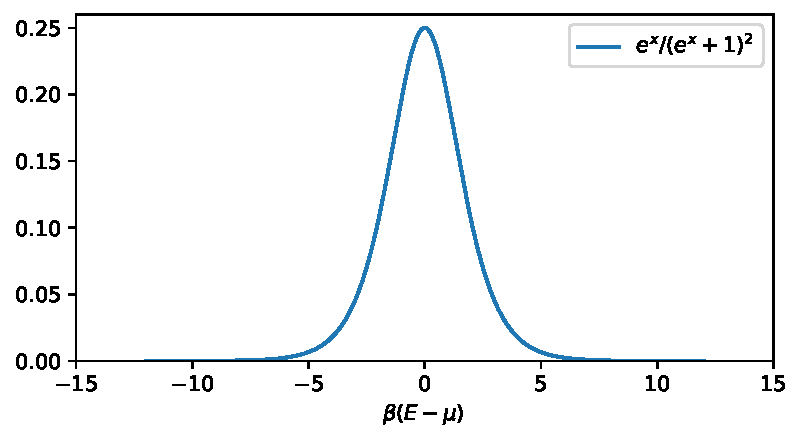
\includegraphics[width=0.5\textwidth]{figs/unit08_Sommerfeld.pdf}\end{center} % WARNING: ADJUSTED SIZE BY HAND TO FILL REMAINDER OF PAGE

These considerations justify two low-temperature approximations.
First, recalling $\mu > 0$ at low temperatures, for large \be we are free to extend the lower limit of the integral to obtain a more convenient domain of integration,
\begin{equation*}
  \vev{N}_{\text{f}} = \frac{2}{3} g_0 \int_{-\be\mu}^{\infty} \frac{e^x}{\left(e^x + 1\right)^2} E^{3 / 2} \; dx \approx \frac{2}{3} g_0 \int_{-\infty}^{\infty} \frac{e^x}{\left(e^x + 1\right)^2} E^{3 / 2} \; dx.
\end{equation*}
Second, we can expand $E^{3 / 2}$ in a Taylor series around $E = \mu$, and truncate after the first few terms:
\begin{align*}
  E^{3 / 2} & \approx \mu^{3 / 2} + (E - \mu) \left. \pderiv{}{E} E^{3 / 2}\right|_{E = \mu} + \frac{1}{2} (E - \mu)^2 \left. \ppderiv{}{E} E^{3 / 2}\right|_{E = \mu} \\
            & = \mu^{3 / 2} + \frac{3}{2} (E - \mu) \mu^{1 / 2} + \frac{3}{8} (E - \mu)^2 \mu^{-1 / 2} = \mu^{3 / 2} + \frac{3}{2} \frac{x \mu^{1 / 2}}{\be} + \frac{3}{8} \frac{x^2 \mu^{-1 / 2}}{\be^2}.
\end{align*}

Switching to work with $T = 1 / \be$, the Sommerfeld expansion has given us a series of manageable integrals we can consider one by one:
\begin{equation*}
  \vev{N}_{\text{f}} \approx \frac{2}{3} g_0 \mu^{3 / 2} \Ibb_1 + g_0 T \mu^{1 / 2} \Ibb_2 + \frac{g_0 T^2}{4\mu^{1 / 2}} \Ibb_3.
\end{equation*}
\begin{mdframed}
  $\displaystyle \Ibb_1 = \int_{-\infty}^{\infty} \frac{e^x}{\left(e^x + 1\right)^2} \; dx = $ \\[80 pt]
  $\displaystyle \Ibb_2 = \int_{-\infty}^{\infty} \frac{x e^x}{\left(e^x + 1\right)^2} \; dx = $ \\[80 pt]
  $\displaystyle \Ibb_3 = \int_{-\infty}^{\infty} \frac{x^2 e^x}{\left(e^x + 1\right)^2} \; dx = $ \\[110 pt] % WARNING: ADJUSTED SIZE BY HAND TO FILL REMAINDER OF PAGE
\end{mdframed}
Collecting the results and restoring $g_0 = V \frac{\sqrt{2m^3}}{\pi^2 \hbar^3}$, you should find
\begin{equation*}
  \vev{N}_{\text{f}} \approx \frac{2}{3} g_0 \mu^{3 / 2} + g_0 \frac{\pi^2 T^2}{12\mu^{1 / 2}} = V \frac{(2m\mu)^{3 / 2}}{3\pi^2\hbar^3} + V \frac{\sqrt{2m^3}}{12\hbar^3 \mu^{1 / 2}} T^2.
\end{equation*}
The first term reproduces what we found with the step-function approximation in \secref{sec:fermi_lowT}, while the second term provides the promised temperature dependence, at leading order in the Sommerfeld expansion.
This becomes more interesting if we rearrange \eq{eq:Fermi_energy} to work in terms of the Fermi energy:
\begin{mdframed}
  $\displaystyle E_F = \frac{\hbar^2}{2m}\left(\frac{3\pi^2 \vev{N}_{\text{f}}}{V}\right)^{2 / 3} \Lra $ \\[120 pt]
\end{mdframed}

The result
\begin{equation*}
  \frac{\mu}{E_F} \approx \left[1 - \frac{\pi^2 T^2}{8 E_F^{3 / 2} \mu^{1 / 2}}\right]^{2 / 3}
\end{equation*}
can be simplified through one final low-temperature approximation.
Because $T$ is small, just in the second term above we can set $E_F \approx \mu$ (the zero-temperature relation).
Then
\begin{equation}
  \label{eq:mu_vs_T}
  \frac{\mu}{E_F} \approx 1 - \frac{\pi^2 T^2}{12 E_F^2},
\end{equation}
which confirms our earlier claim $\mu \leq E_F$, and reveals that the leading correction to the zero-temperature relation is quadratic in $T$.

The calculation is essentially the same for the internal energy from \eq{eq:DoS_full}.
With $E^{3 / 2}$ in place of $E^{1 / 2}$, integrating by parts just gives
\begin{equation*}
  \vev{E}_{\text{f}} = g_0 \int_0^{\infty} \frac{E^{3 / 2}}{e^{\be(E - \mu)} + 1} dE \approx \frac{2}{5} g_0 \int_{-\infty}^{\infty} \frac{e^x}{\left(e^x + 1\right)^2} E^{5 / 2} \; dx
\end{equation*}
with the same $x = \be(E - \mu)$ and extended lower limit of integration.
The Taylor expansion
\begin{equation*}
  E^{5 / 2} \approx \mu^{5 / 2} + \frac{5}{2} (E - \mu) \mu^{3 / 2} + \frac{15}{8} (E - \mu)^2 \mu^{1 / 2} = \mu^{5 / 2} + \frac{5}{2} \frac{x \mu^{3 / 2}}{\be} + \frac{15}{8} \frac{x^2 \mu^{1 / 2}}{\be^2}
\end{equation*}
also produces the same integrals, with different coefficients:
\begin{equation*}
  \vev{E}_{\text{f}} \approx \frac{2}{5} g_0 \mu^{5 / 2} \Ibb_1 + g_0 T \mu^{3 / 2} \Ibb_2 + \frac{3}{4} g_0 T^2 \mu^{1 / 2} \Ibb_3 = \frac{2}{5} g_0 \mu^{5 / 2} + \frac{1}{4} g_0 \pi^2 T^2 \mu^{1 / 2}.
\end{equation*}
Inserting $g_0 = \frac{3\vev{N}_{\text{f}}}{2E_F^{3 / 2}}$, we have
\begin{equation*}
  \vev{E}_{\text{f}} \approx \frac{3}{5} \vev{N}_{\text{f}} \frac{\mu^{5 / 2}}{E_F^{3 / 2}} + \frac{3}{8} \vev{N}_{\text{f}} \pi^2 T^2 \frac{\mu^{1 / 2}}{E_F^{3 / 2}},
\end{equation*}
which we can simplify by applying \eq{eq:mu_vs_T} and dropping $\cO\left(T^3\right)$ terms:
\begin{mdframed}
  $\displaystyle \mu^{5 / 2} \approx $ \\[100 pt]
\end{mdframed}
From your result you should obtain the heat capacity
\begin{equation*}
  c_v = \left. \pderiv{}{T} \vev{E} \right|_{N,V} \approx \frac{\pi^2}{2} \frac{\vev{N}_{\text{f}}}{E_F} T.
\end{equation*}
This low-temperature linear dependence on $T$ agrees with experimental heat capacity measurements, as we will see in the next tutorial.

As a final comment in this supplement, let's consider what would happen to $\vev{N}_{\text{f}}$ at higher temperatures $T^2 \sim E_F^2$, for which the two terms in \eq{eq:mu_vs_T} would cancel out, leaving $\cO(T^4 / E_F^4)$ effects non-negligible.
In this regime, there's no guarantee that the low-temperature Sommerfeld expansion would even converge, so we need to work with the full integral from \eq{eq:DoS_full}.
Fortunately, it is not hard to numerically evaluate this integral, which is done by \href{https://github.com/daschaich/MATH327_2022/blob/master/lecture_notes/unit08_fermi-gas.py}{this Python code}.
For the purpose of numerical analysis, it's best to express everything in terms of dimensionless ratios, such as
\begin{align*}
  t & \equiv \frac{T}{E_F} \qquad &
  c & \equiv \frac{\mu}{E_F} \qquad &
  x & \equiv \frac{E}{T} = \be E.
\end{align*}
Also inserting $g_0 = \frac{3\vev{N}_{\text{f}}}{2E_F^{3 / 2}}$, we have
\begin{equation*}
  \vev{N}_{\text{f}} = \frac{3\vev{N}_{\text{f}}}{2E_F^{3 / 2}} \int_0^{\infty} \frac{\sqrt{E}}{e^{\be(E - \mu)} + 1} dE = \frac{3\vev{N}_{\text{f}}}{2} t^{3 / 2} \int_0^{\infty} \frac{\sqrt{x} e^{-x}}{e^{-c / t} + e^{-x}} dx,
\end{equation*}
working with small $e^{-\be E} = e^{-x}$ rather than large $e^x$ to avoid numerical overflow.

As in \eq{eq:mu_vs_T}, $\vev{N}_{\text{f}}$ drops out, and we end up with the consistency condition
\begin{equation}
  1 = \frac{3}{2} t^{3 / 2} \int_0^{\infty} \frac{\sqrt{x} e^{-x}}{e^{-c / t} + e^{-x}} dx.
\end{equation}
If we fix the temperature $t = T / E_F$ in units of the Fermi energy, by repeatedly evaluating this integral with different values of $c = \mu / E_F$ we can determine the self-consistent value of the chemical potential, also in units of the Fermi energy.
The red $\times$'s in the figure below are results of such work for eleven temperatures $0.1 \leq t \leq 2$, compared to the $\cO\left(t^2\right)$ result from the Sommerfeld expansion, \eq{eq:mu_vs_T}.
This leading-order Sommerfeld expansion clearly deviates from the full results by the time $T \sim E_F$.
The more interesting result is that the chemical potential continues to decrease as the temperature increases, becoming negative for $T \gtrsim E_F$ and approaching the expected high-temperature classical limit.

\begin{center}\noindent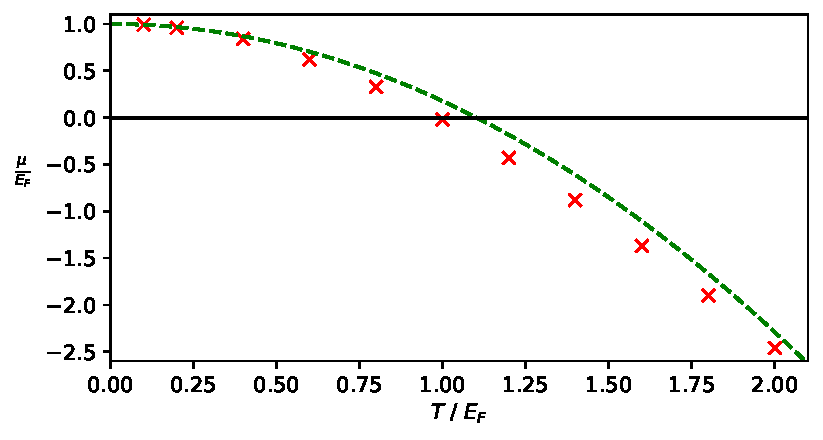
\includegraphics[width=0.8\textwidth]{figs/unit08_fermi-gas.pdf}\end{center}
% ------------------------------------------------------------------
